\documentclass{beamer}
\usepackage{verbatim}
\usepackage{amsmath}
\usepackage{amssymb}
\usepackage{epsfig}
\usepackage{subfigure}
\usepackage{multirow}
\usepackage{color}
\usepackage{float}
\usepackage{hyperref}
\usepackage{graphics}
\usepackage{graphicx}
\usepackage{rotating}
\usetheme{Boadilla}
\usecolortheme{rose}
\usepackage[percent]{overpic}
\usefonttheme{structureitalicserif}
\setbeamercovered{invisible}
\setbeamertemplate{navigation symbols}{}
\usepackage{epstopdf}
\usepackage{adjustbox}

\title[Weak-lensing magnification]{Weak-lensing magnification\\ as a probe for the dark Universe}
\author[M. Garcia-Fernandez]{M. Garcia-Fernandez}
\institute[CIEMAT]{{\bf CIEMAT}}
\date[October 30th, 2017]{October 30th, 2017}
\begin{document}
%%%%%%%%%%%%%%%%%%%%%%%%%%%%%%%%%%%%%%%%%%%%%%%%%%%%%%%%%%%%%%%%%%%%%
\begin{frame}[plain]
\maketitle
\begin{center}

\includegraphics[trim={0 0 6cm 0},clip=True,height=26pt]{./figures/logomaetzu.png}
\end{center}
\end{frame}
%%%%%%%%%%%%%%%%%%%%%%%%%%%%%%%%%%%%%%%%%%%%%%%%%%%%%%%%%%%%%%%%%%%%%%%%%
\begin{frame}
\frametitle{\begin{small}\underline{{\bf The dark Universe.}}\end{small}}
\begin{center}
\begin{overpic}[height=0.5\textheight]{./sky_mechanics.jpg}
\put(-40,10){\rotatebox{45}{\colorbox{white}{$R_{\mu\nu}-\frac{1}{2}Rg_{\mu\nu}+\Lambda g_{\mu\nu}=\frac{8\pi G_N}{c^4}T_{\mu\nu}$}}}
\end{overpic}
\end{center}
\end{frame}
%%%%%%%%%%%%%%%%%%%%%%%%%%%%%%%%%%%%%%%%%%%%%%%%%%%%%%%%%%%%%%%%%%%%%%%%%
\begin{frame}
\frametitle{\begin{small}\underline{{\bf The dark Universe.}}\end{small}}
\begin{columns}
\column{0.5\textwidth}
\begin{center}
{\bf CMB}\\
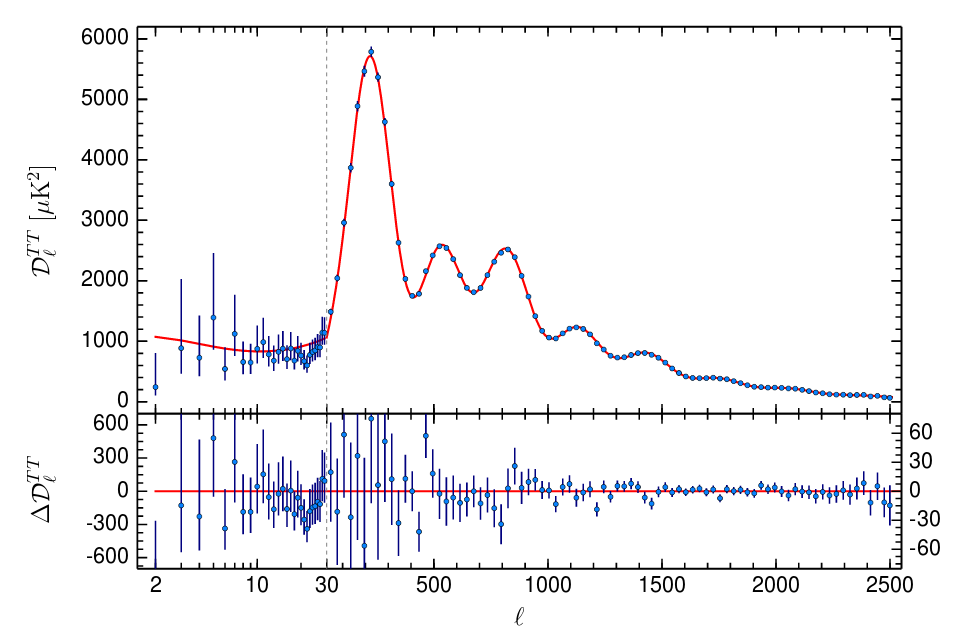
\includegraphics[width=0.6\textwidth]{./CMB_pk.png}\\
{\bf Accelerated expansion}\\
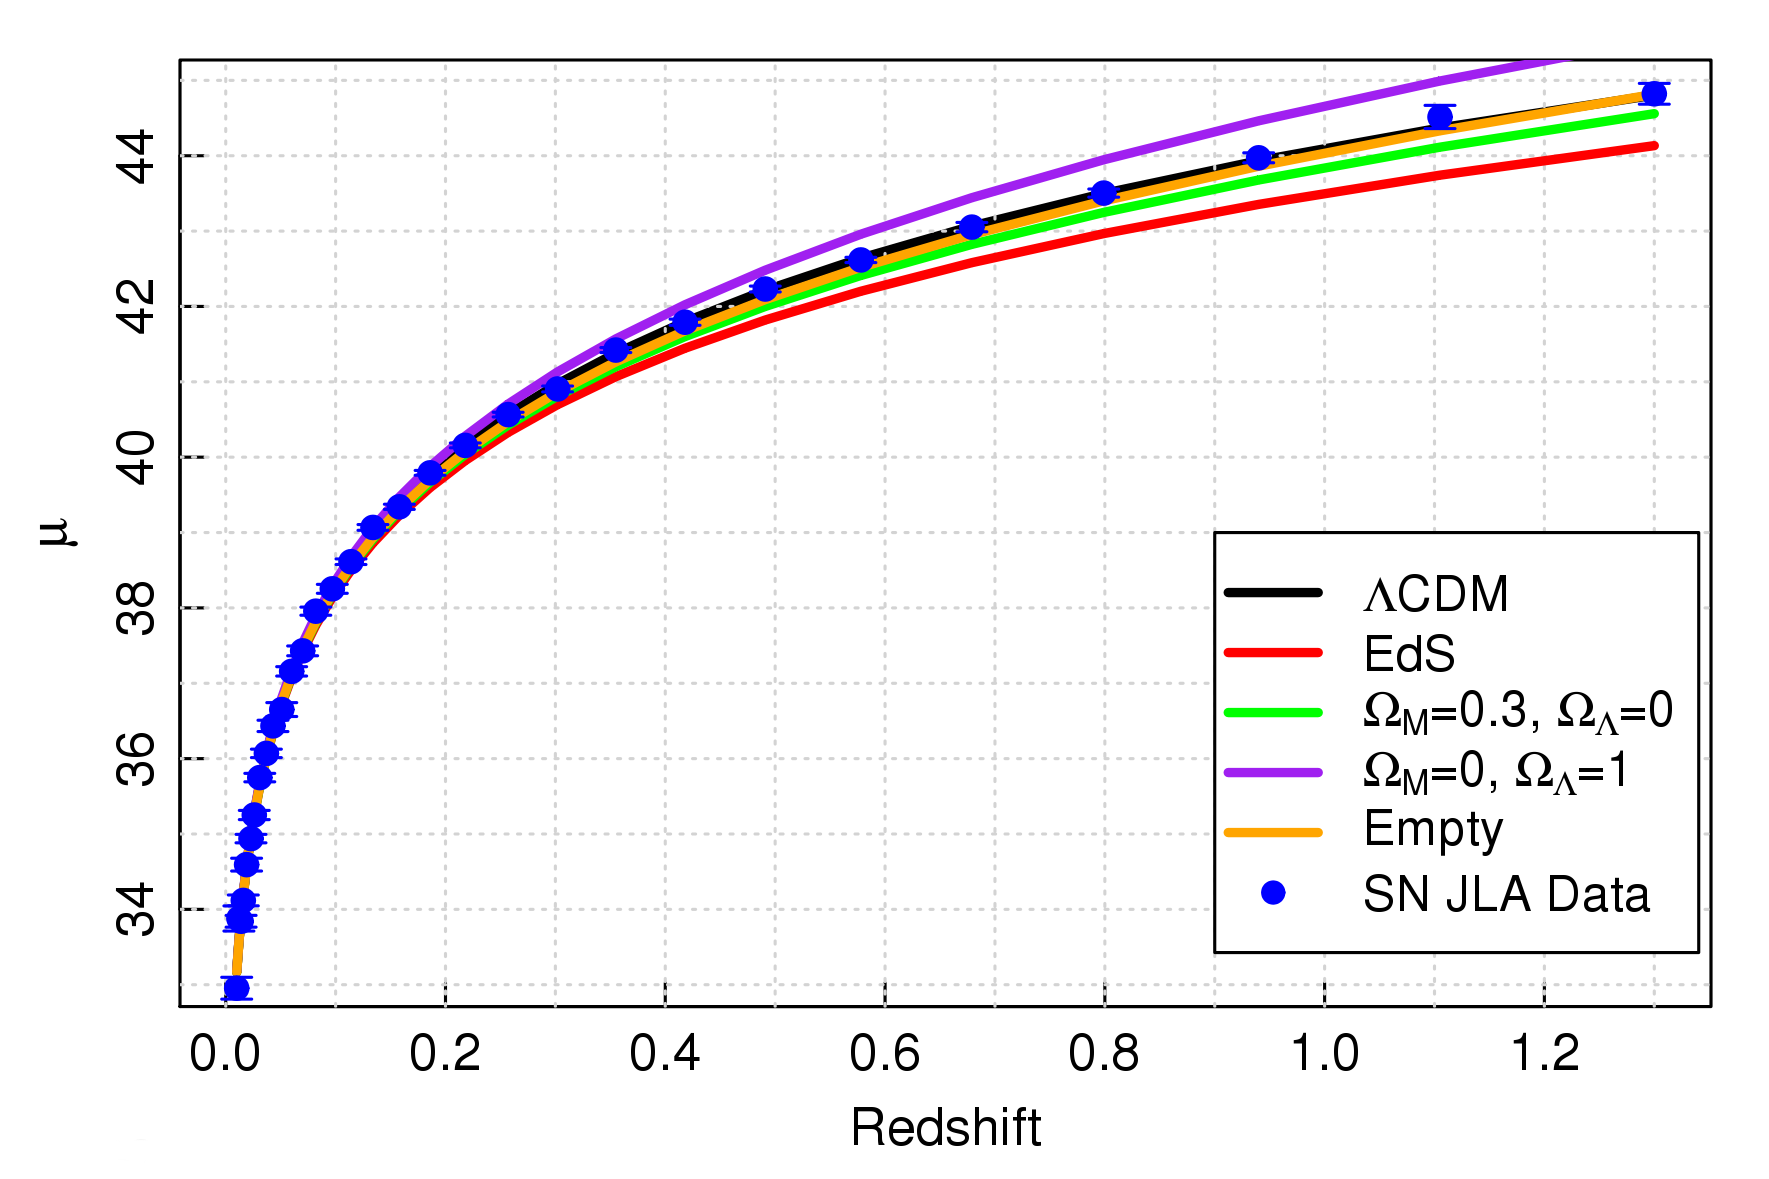
\includegraphics[width=0.6\textwidth]{./distance_modulus.png}\\
\end{center}
\column{0.5\textwidth}
\begin{center}
{\bf BAO}\\
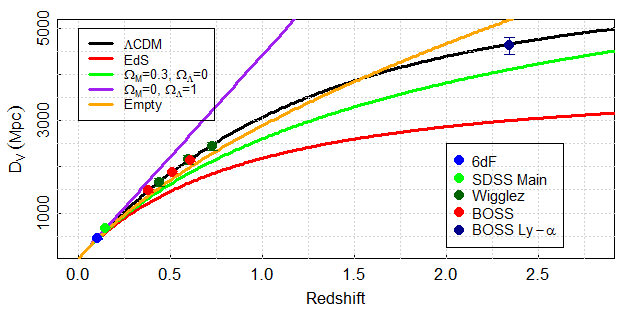
\includegraphics[width=0.8\textwidth]{./bao_dv.png}\\
{\bf Primordial Nucleosynthesis}\\
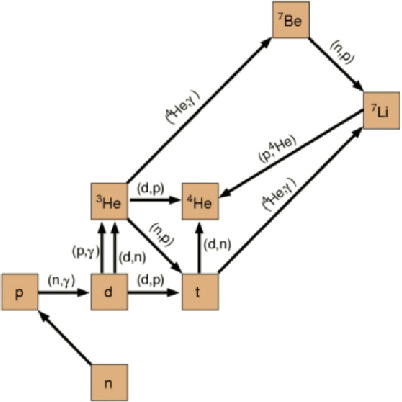
\includegraphics[width=0.5\textwidth]{./BBN.png}\\
\end{center}
\end{columns}
\end{frame}
%%%%%%%%%%%%%%%%%%%%%%%%%%%%%%%%%%%%%%%%%%%%%%%%%%%%%%%%%%%%%%%%%%%%%%%%%
\begin{frame}
\frametitle{\begin{small}\underline{{\bf The dark Universe.}}\end{small}}
\begin{columns}
\column{0.4\textwidth}
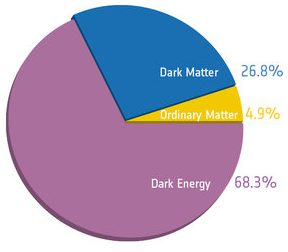
\includegraphics[width=\textwidth]{./cosmic_pie.jpg}
\column{0.6\textwidth}
{\color{red}{\bf Only the 5\% of the Universe is known}}\\
\vspace*{1cm}
Dark Energy: Responsible of the acceleration.\\
\vspace*{1cm}
Dark matter: Only interacts through gravity.
\end{columns}
\end{frame}
%%%%%%%%%%%%%%%%%%%%%%%%%%%%%%%%%%%%%%%%%%%%%%%%%%%%%%%%%%%%%%%%%%%%%%%%%
\begin{frame}
\frametitle{\begin{small}\underline{{\bf The dark Universe.}}\end{small}}
{\bf Dark Energy as the Cosmological Constant:}\\
$\rightarrow$ Disagreement between Cosmology and HEP-Physics:\\
$$\rho_{\Lambda}\sim 10^{-47}\mbox{ GeV}^4;\ \ \ \rho_{HEP}\sim 246\mbox{ GeV}^4$$\\
\vspace{0.5cm}
{Alternative explanations:}
\begin{itemize}
\item {\bf Exotic quantum fields:} quintessence, k-essence, chamaleon fields...
\vspace{0.2cm}
\item {\bf Modified gravity theories:} $f(R)$, TeVeS, Honderski...
\end{itemize}
\end{frame}
%%%%%%%%%%%%%%%%%%%%%%%%%%%%%%%%%%%%%%%%%%%%%%%%%%%%%%%%%%%%%%%%%%%%%%%%%
\begin{frame}
\frametitle{\begin{small}\underline{{\bf The dark Universe.}}\end{small}}
{\bf Modeling departures from General Relativity:}
\begin{itemize}
\item Equation of state:\\
$$p=wV \Rightarrow w={\bf \color{red}w_0}+(1-a){\bf \color{red}w_a}$$
With $w_0=-1$ and $w_a=0$ for the Cosmological Constant.
\vspace{0.2cm}
\item Departures from the metric $ ds^2 = a^2[-(1+2\Psi)d\tau^2+(1-2\Phi)dx_idx^j]$:\\
$$2\nabla^2\Phi\frac{8\pi G_N}{c^2}a^2{\bf\color{red}\mu}\bar\rho_M\delta_M;\ \ \ {\bf\color{red}\gamma}=\frac{\Phi}{\Psi}$$
With $\mu=\gamma=1$ for general relativity.
\end{itemize}
\end{frame}
%%%%%%%%%%%%%%%%%%%%%%%%%%%%%%%%%%%%%%%%%%%%%%%%%%%%%%%%%%%%%%%%%%%%%%%%%
\begin{frame}
\frametitle{\begin{small}\underline{{\bf The dark Universe.}}\end{small}}
\begin{center}
{\bf Status of dark energy constrains.}
\end{center}
\begin{columns}
\column{0.5\textwidth}
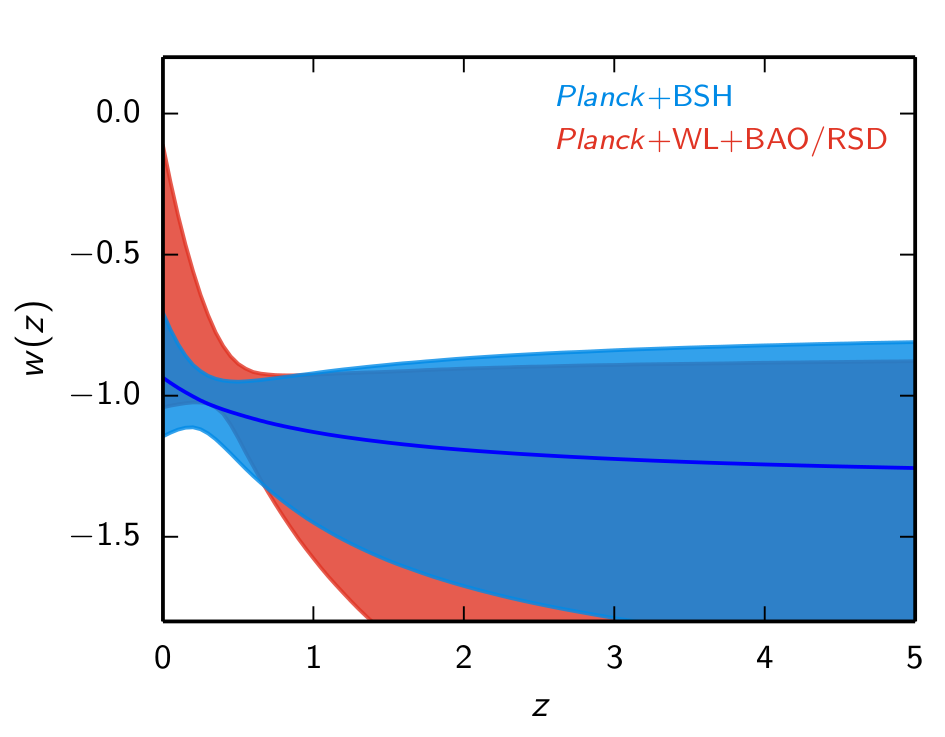
\includegraphics[width=\textwidth]{./equationofstate_planck2015.png}
\column{0.5\textwidth}
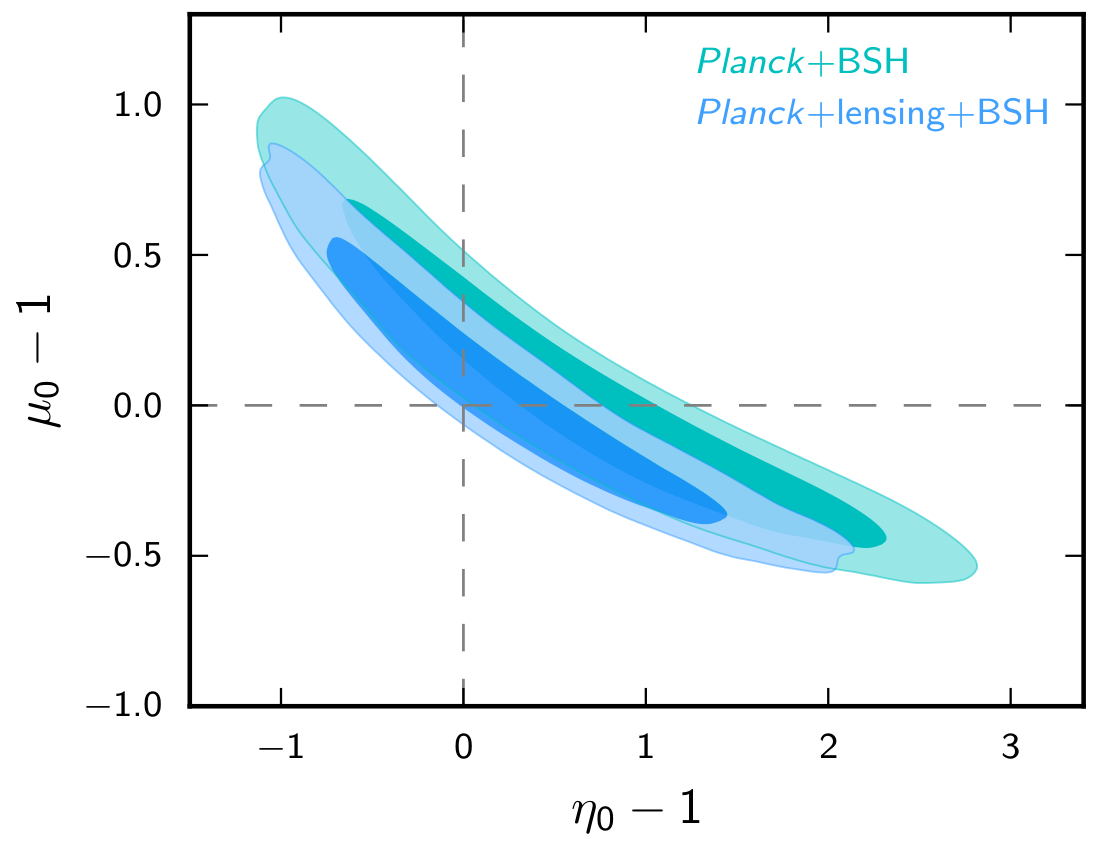
\includegraphics[width=\textwidth]{./mg_planck2015.png}
\end{columns}
\end{frame}
%%%%%%%%%%%%%%%%%%%%%%%%%%%%%%%%%%%%%%%%%%%%%%%%%%%%%%%%%%%%%%%%%%%%%%%%%
\begin{frame}[plain]
\begin{LARGE}
\begin{center}
{{\bf \color{blue}THE DARK ENERGY SURVEY}}
\end{center}
\end{LARGE}
\end{frame}
%%%%%%%%%%%%%%%%%%%%%%%%%%%%%%%%%%%%%%%%%%%%%%%%%%%%%%%%%%%%%%%%%%%%%%%%%
\begin{frame}
\frametitle{\begin{small}\underline{{\bf The Dark Energy Survey.}}\end{small}}
\begin{center}
Dark Energy $\Rightarrow$ Accelerated expansion of the Universe.\\
\vspace{0.5cm}
\color{red}{\bf What is the nature of Dark Energy?}
\end{center}
\begin{columns}
\column{0.5\textwidth}
Combining 4 m\'ethods:
\begin{itemize}
\item Supernovae
\item Cluster
\item BAO
\item \color{red}{\bf Gravitational lensing}
\end{itemize}
\column{0.5\textwidth}
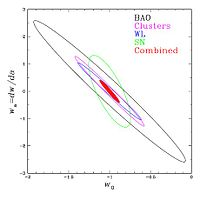
\includegraphics[width=0.8\textwidth]{./fom.jpg}
\end{columns}
\end{frame}
%%%%%%%%%%%%%%%%%%%%%%%%%%%%%%%%%%%%%%%%%%%%%%%%%%%%%%%%%%%%%%%%%%%%%%%%%
\begin{frame}
\frametitle{\begin{small}\underline{{\bf The Dark Energy Survey.}}\end{small}}
\begin{columns}
\column{0.7\textwidth}
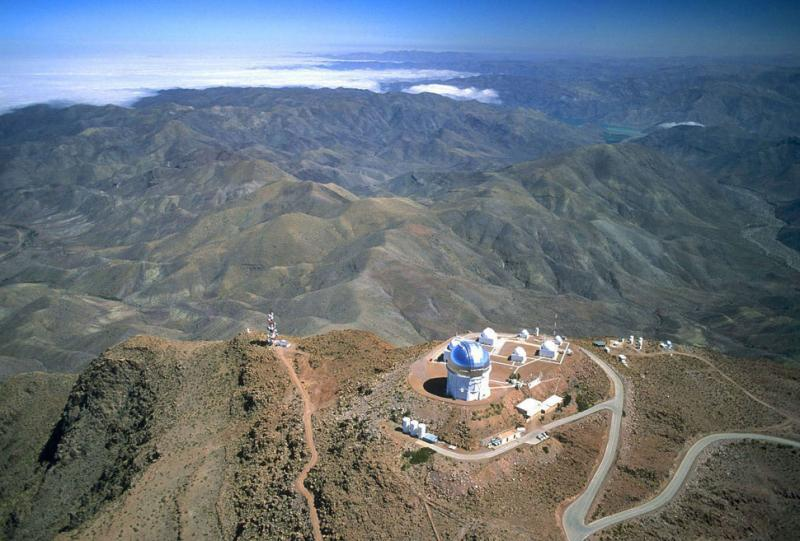
\includegraphics[width=\textwidth]{./cerrotololo.jpg}
\column{0.3\textwidth}
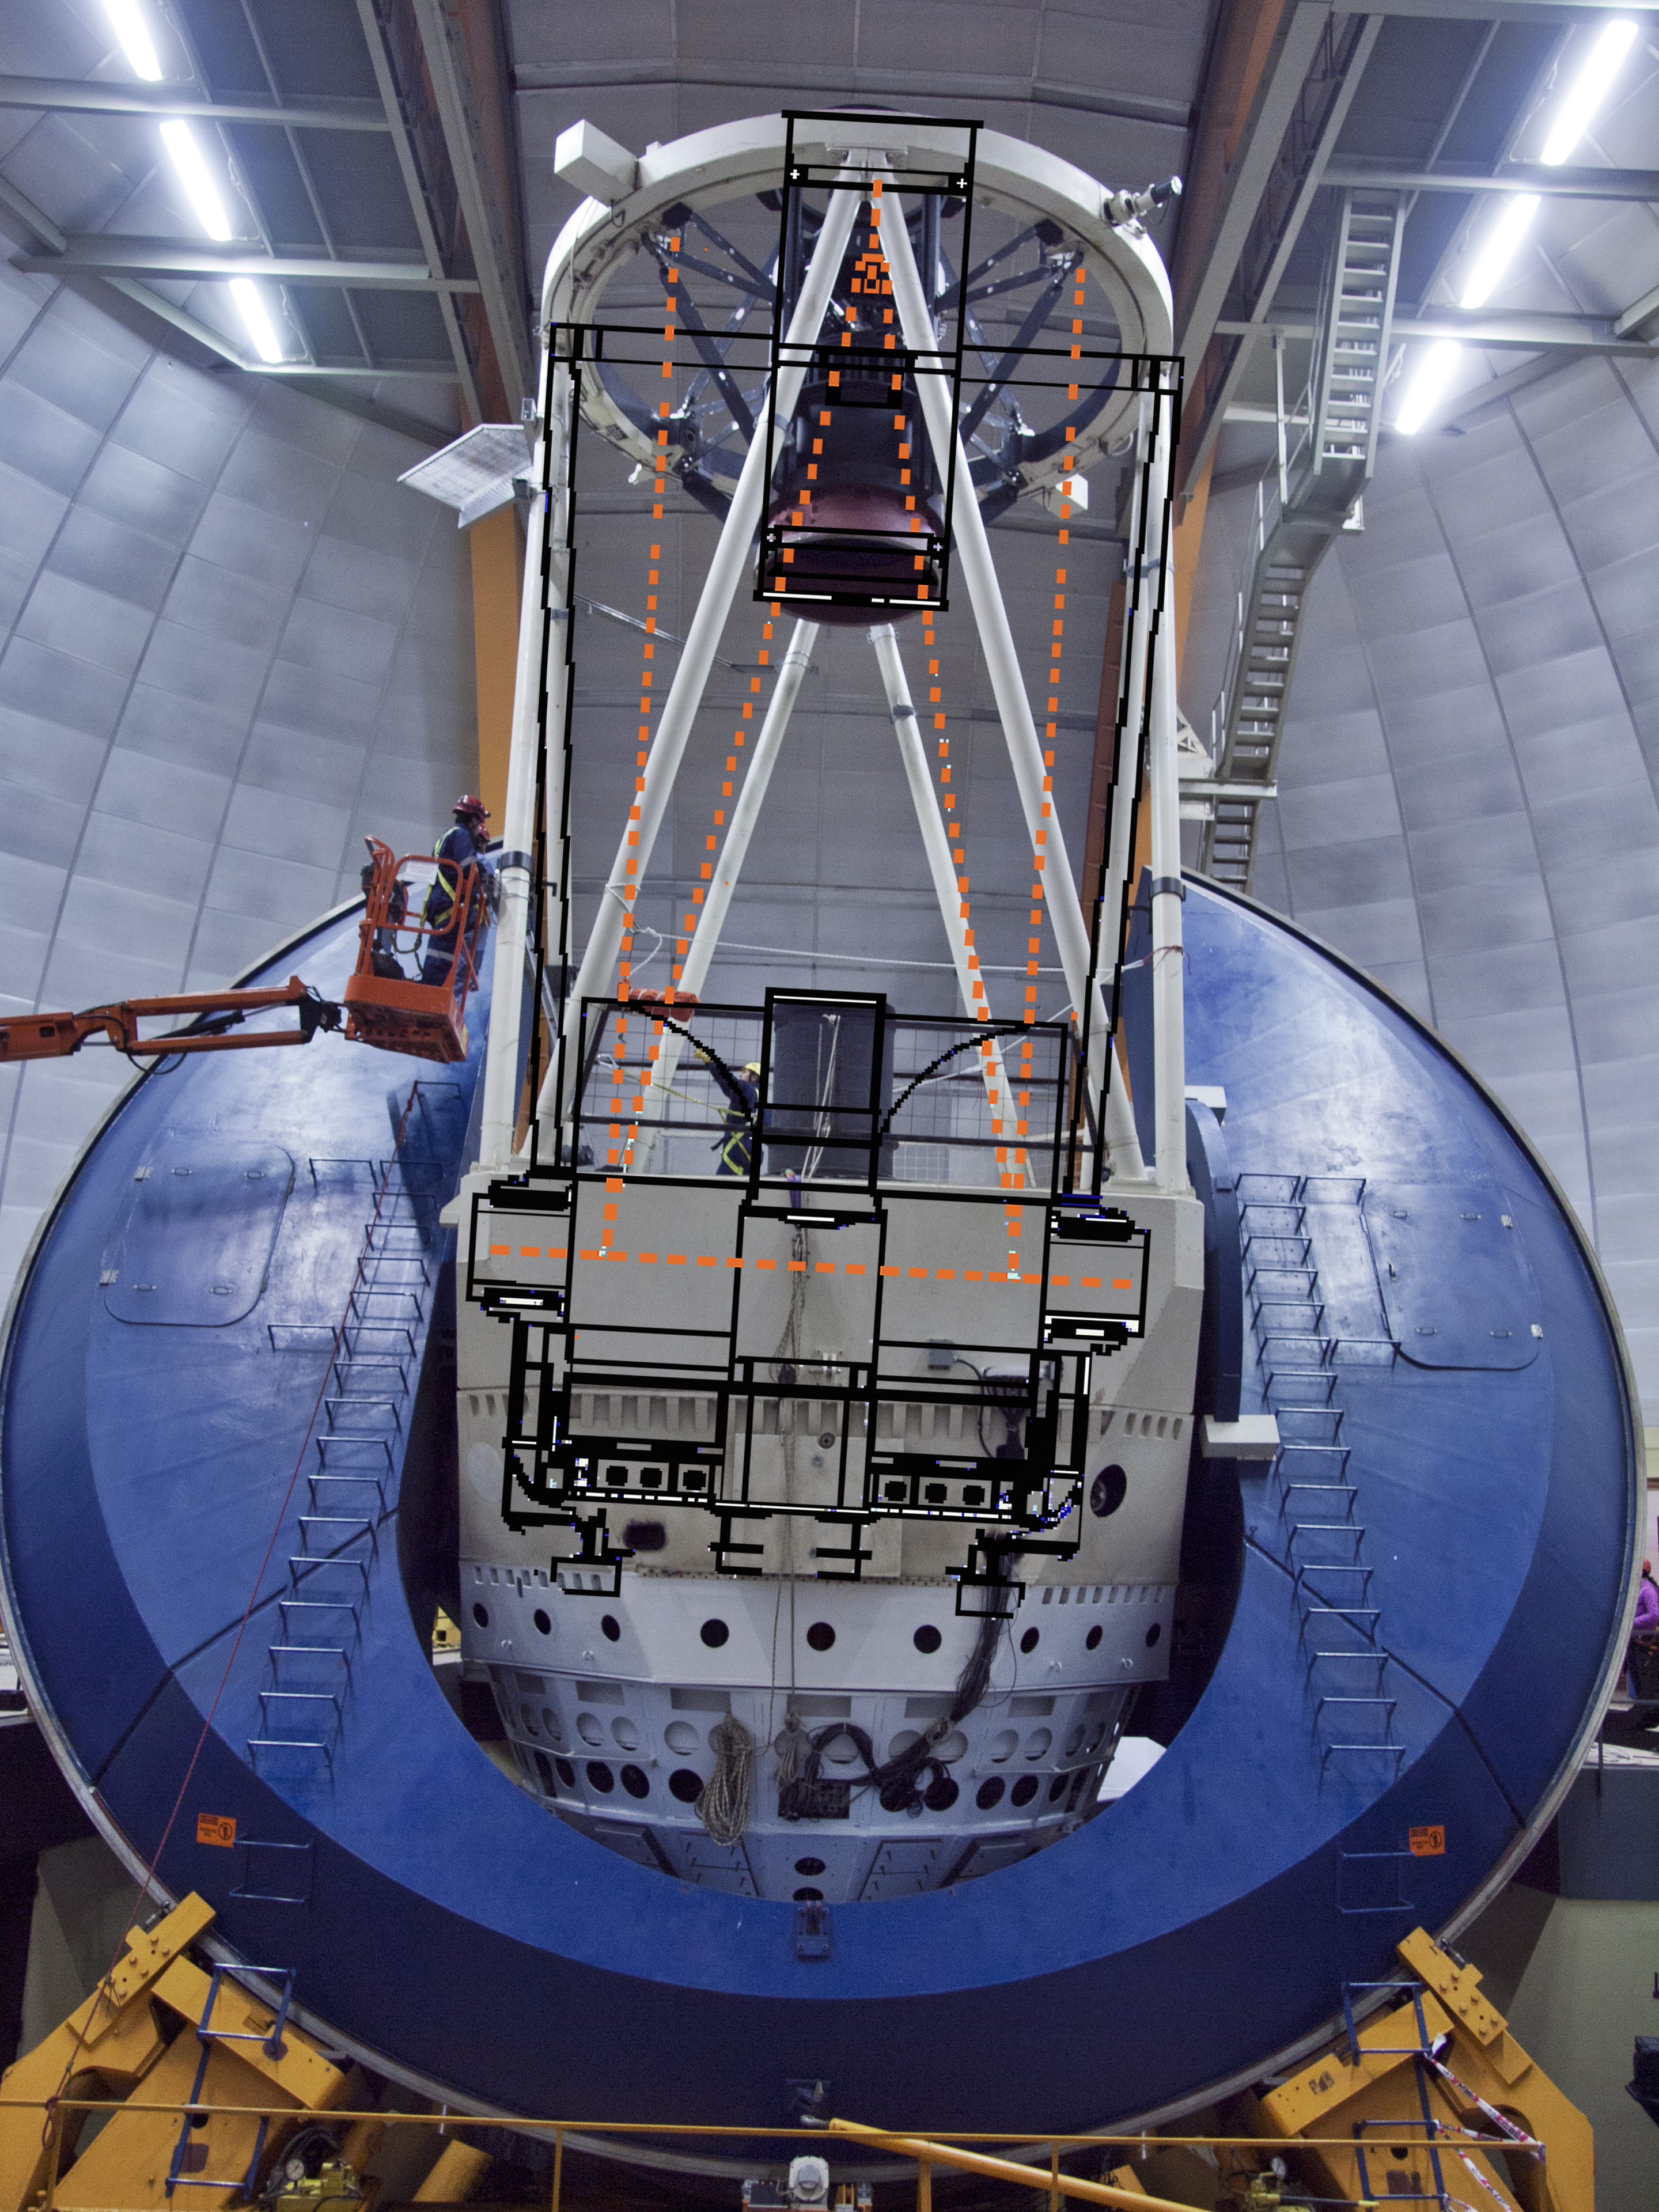
\includegraphics[width=\textwidth]{./decam.jpg}\\
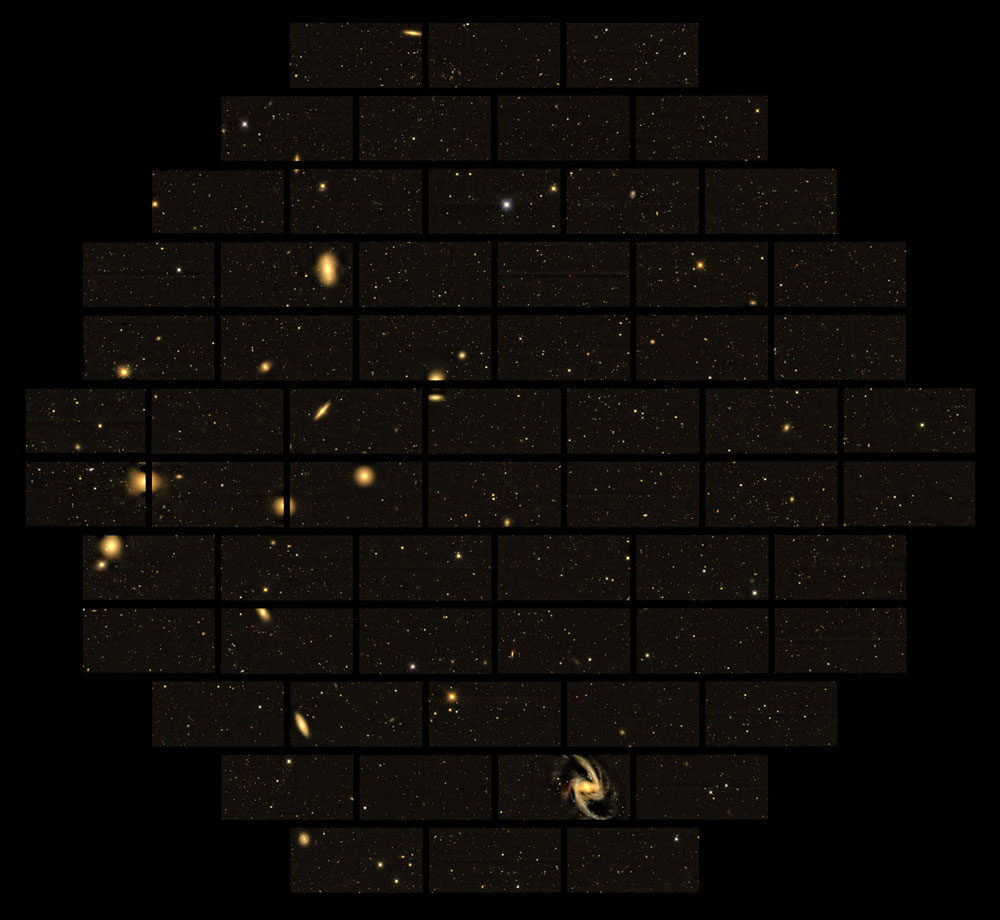
\includegraphics[width=\textwidth]{./decam-fov.jpg}
\end{columns}
\end{frame}
%%%%%%%%%%%%%%%%%%%%%%%%%%%%%%%%%%%%%%%%%%%%%%%%%%%%%%%%%%%%%%%%%%%%%%%%%
\begin{frame}
\frametitle{\begin{small}\underline{{\bf The Dark Energy Survey.}}\end{small}}
\begin{center}
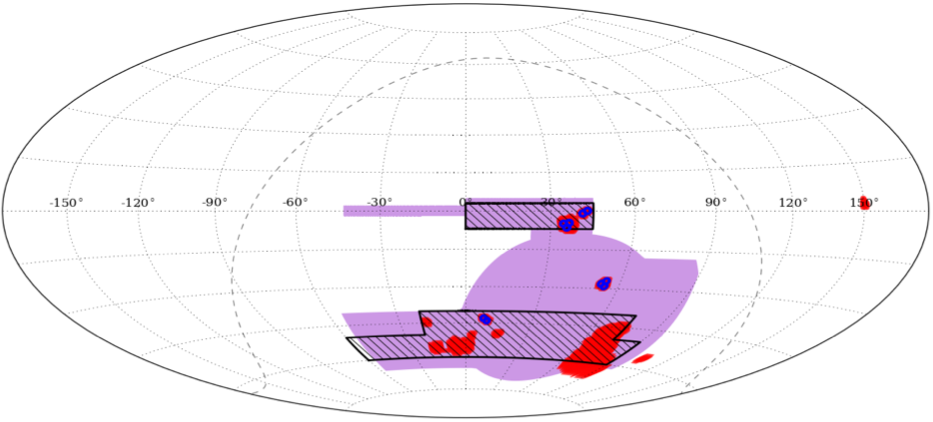
\includegraphics[width=0.6\textwidth]{./des_footprint.png}
\end{center}
\begin{columns}
\column{0.5\textwidth}
\begin{itemize}
\item Photometric survey.
\item SV \& Y1-Y4 done.
\item Total de 5 campaigns.
\end{itemize}
\column{0.5\textwidth}
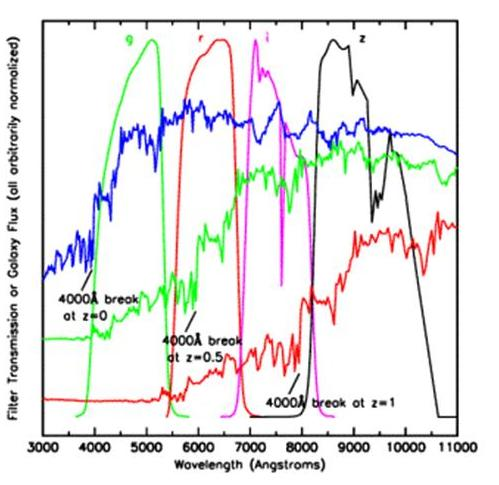
\includegraphics[width=0.6\textwidth]{./des-filters.jpg}
\end{columns}
\end{frame}
%%%%%%%%%%%%%%%%%%%%%%%%%%%%%%%%%%%%%%%%%%%%%%%%%%%%%%%%%%%%%%%%%%%%%%%%%
\begin{frame}
\frametitle{\begin{small}\underline{{\bf The Dark Energy Survey.}}\end{small}}
\begin{center}
{\bf Where are we now?}\\
\vspace{0.2cm}
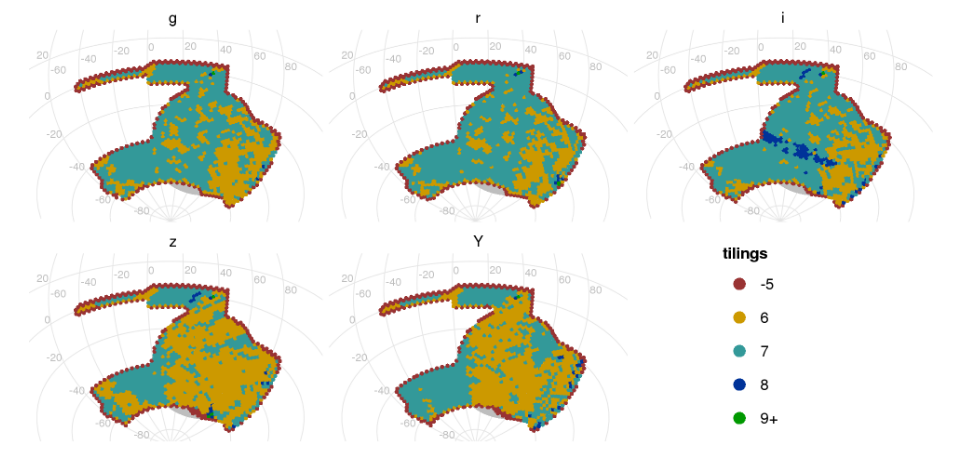
\includegraphics[width=0.8\textwidth]{./des_tiles.png}
\end{center}
\end{frame}
%%%%%%%%%%%%%%%%%%%%%%%%%%%%%%%%%%%%%%%%%%%%%%%%%%%%%%%%%%%%%%%%%%%%%%%%%
\begin{frame}
\frametitle{\begin{small}\underline{{\bf The Dark Energy Survey.}}\end{small}}
\begin{center}
{\bf \color{red} Latest cosmological results: Y1 clustering + lensing}\\
\vspace{0.2cm}
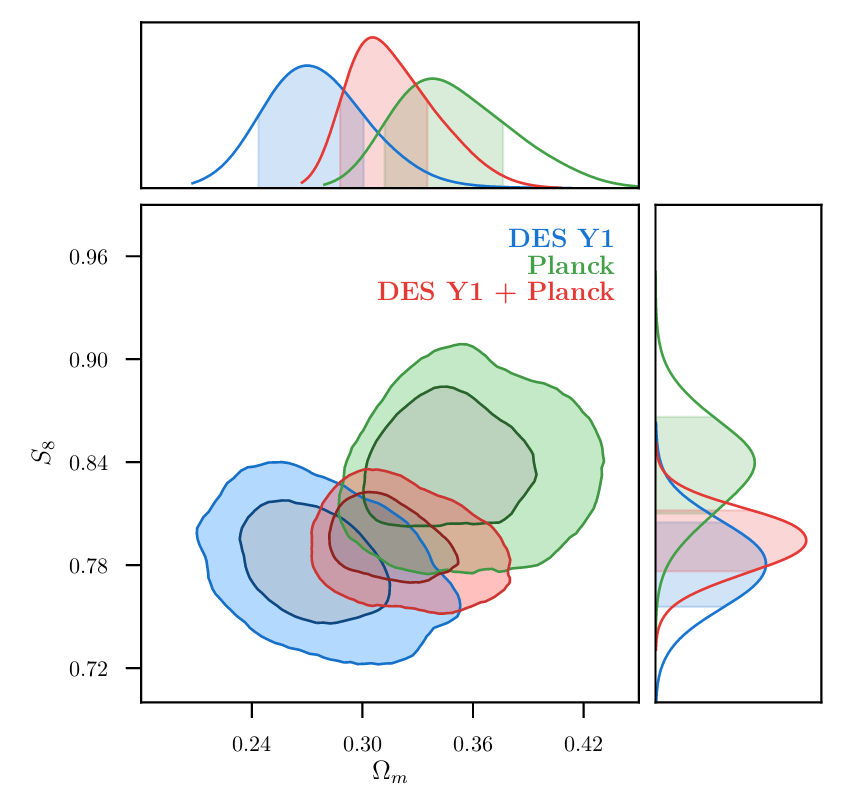
\includegraphics[width=0.6\textwidth]{./des_y1_result.png}
\end{center}
\end{frame}
%%%%%%%%%%%%%%%%%%%%%%%%%%%%%%%%%%%%%%%%%%%%%%%%%%%%%%%%%%%%%%%%%%%%%%%%%
\begin{frame}
\frametitle{\begin{small}\underline{{\bf The Dark Energy Survey.}}\end{small}}
\begin{center}
{\bf Ancillary science: Dark-matter annihilation from dSph.}\\
\vspace{0.2cm}
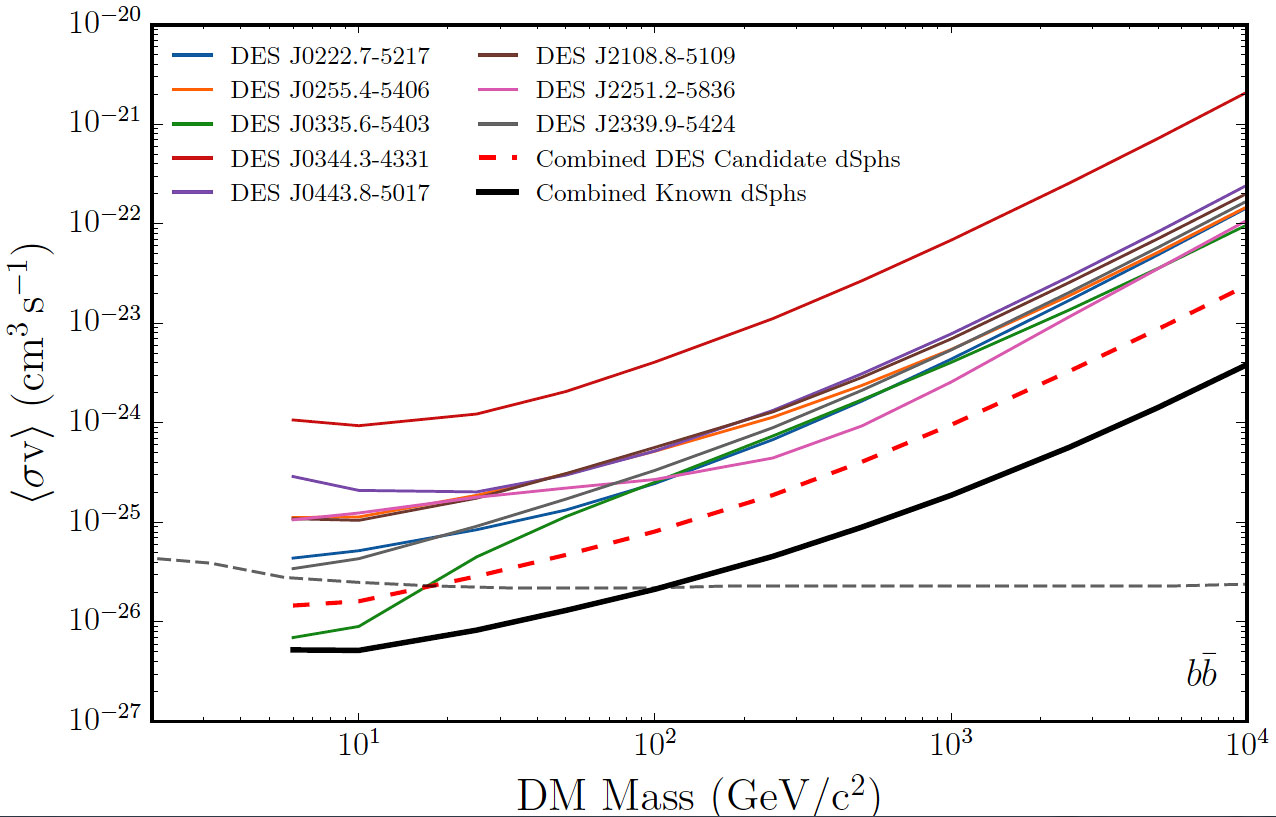
\includegraphics[width=0.8\textwidth]{./dark_matter_anihilation.jpg}
\end{center}
\end{frame}
%%%%%%%%%%%%%%%%%%%%%%%%%%%%%%%%%%%%%%%%%%%%%%%%%%%%%%%%%%%%%%%%%%%%%%%%%
\begin{frame}
\frametitle{\begin{small}\underline{{\bf The Dark Energy Survey.}}\end{small}}
\begin{center}
{\bf Ancillary science: Solar-system astronomy.}\\
\vspace{0.2cm}
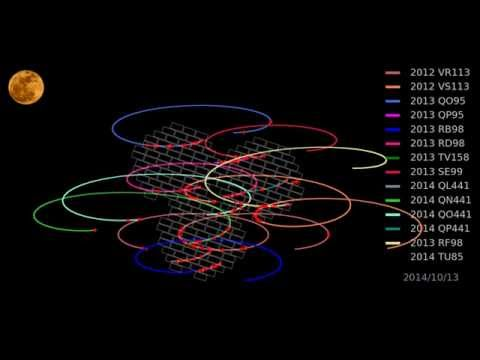
\includegraphics[width=0.6\textwidth]{./TNOS.jpg}
\end{center}
\end{frame}
%%%%%%%%%%%%%%%%%%%%%%%%%%%%%%%%%%%%%%%%%%%%%%%%%%%%%%%%%%%%%%%%%%%%%%%%%
\begin{frame}[plain]
\begin{LARGE}
\begin{center}
{{\bf \color{blue}GRAVITATIONAL LENSING}}
\end{center}
\end{LARGE}
\end{frame}
%%%%%%%%%%%%%%%%%%%%%%%%%%%%%%%%%%%%%%%%%%%%%%%%%%%%%%%%%%%%%%%%%%%%%%%%%
\begin{frame}
\frametitle{\begin{small}\underline{{\bf Gravitational lensing.}}\end{small}}
\begin{columns}
\column{0.5\textwidth}
\begin{center}
General Relativity.
$$\Downarrow$$
Matter curls space-time.
$$\Downarrow$$
Gravity influences photons:\\
light `weights'.
\end{center}
\column{0.5\textwidth}
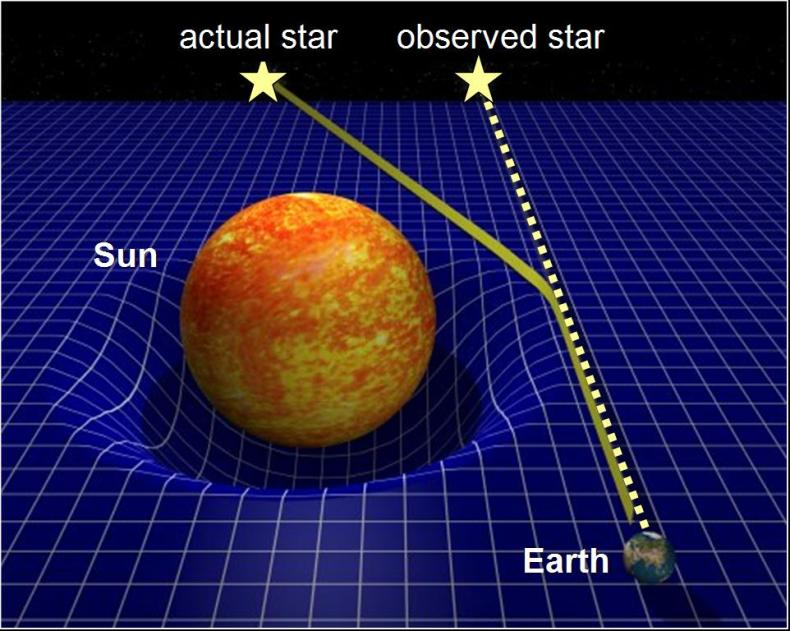
\includegraphics[width=0.9\textwidth]{./light_bending.jpg}\\
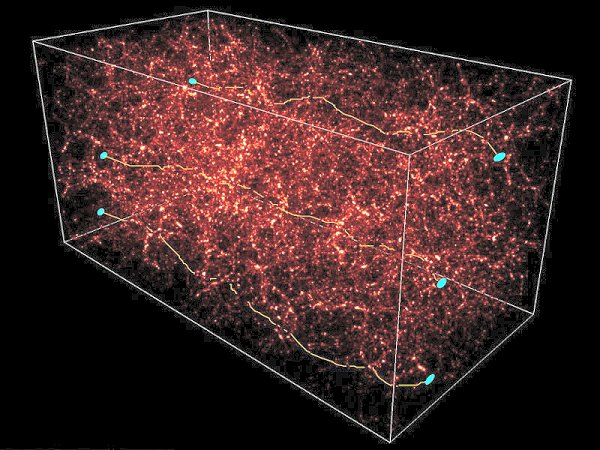
\includegraphics[width=0.9\textwidth]{./universelensing.jpg}
\end{columns}
\end{frame}
%%%%%%%%%%%%%%%%%%%%%%%%%%%%%%%%%%%%%%%%%%%%%%%%%%%%%%%%%%%%%%%%%%%%%%%%%
\begin{frame}
\frametitle{\begin{small}\underline{{\bf Gravitational lensing.}}\end{small}}
\begin{columns}
\column{0.5\textwidth}
\begin{center}
Specific case:\\
Strong field regime.
$$\Downarrow$$
Einstein Rings.
\end{center}
\column{0.5\textwidth}
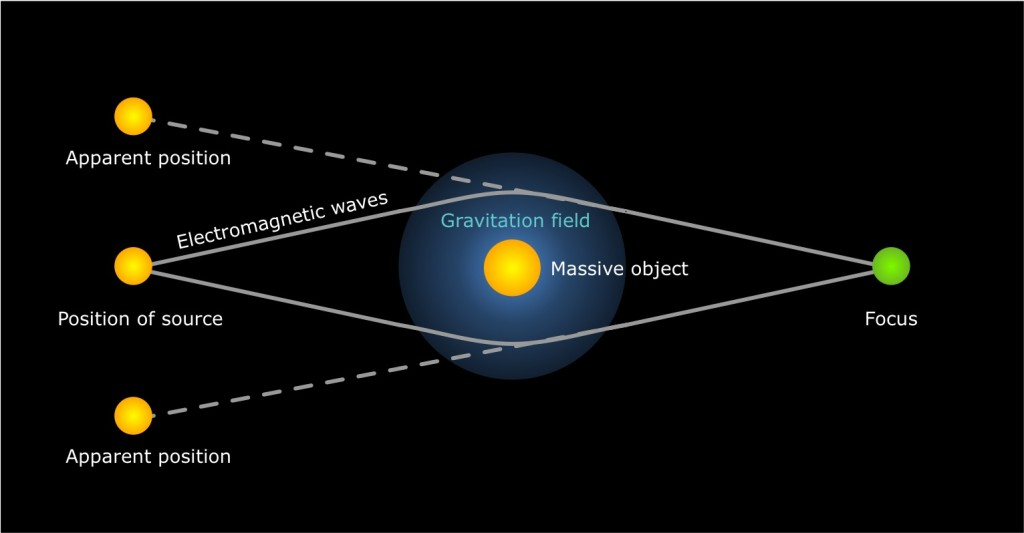
\includegraphics[width=\textwidth]{./strong_lens_diagram.jpg}\\
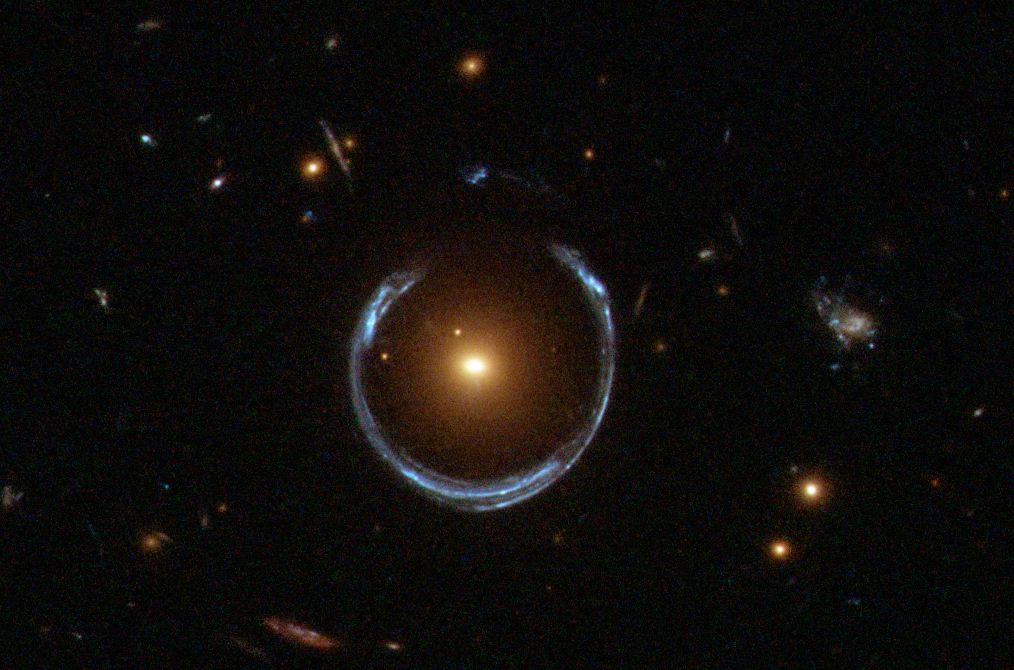
\includegraphics[width=\textwidth]{./strong_lens_picture.jpg}
\end{columns}
\end{frame}
%%%%%%%%%%%%%%%%%%%%%%%%%%%%%%%%%%%%%%%%%%%%%%%%%%%%%%%%%%%%%%%%%%%%%%%%%
\begin{frame}
\frametitle{\begin{small}\underline{{\bf Gravitational lensing.}}\end{small}}
\begin{columns}
\column{0.5\textwidth}
{\bf \underline{Point mass} }\\
\vspace{0.2cm}
Deflection angle: $\alpha = \frac{4GM}{c^2r}\hat r$\\
\vspace{0.5cm}
{\bf \underline{Continuous field} }\\
\vspace{0.2cm}
$\vec\alpha(\hat n) = \frac{1}{\pi}\int d^2\vec r_\perp' \frac{\Sigma(\vec r_\perp')}{\Sigma_c}\frac{\vec r_\perp-\vec r_\perp'}{|\vec r_\perp-\vec r_\perp'|^2}$\\
\column{0.5\textwidth}
\begin{center}
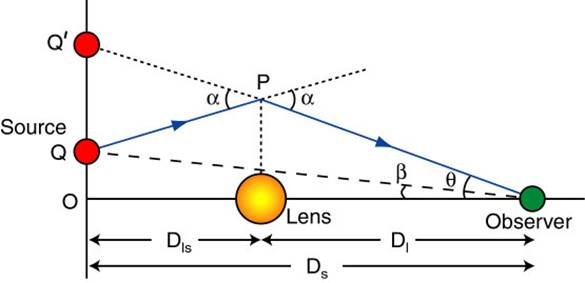
\includegraphics[width=\textwidth]{./figures/gravitational_lens.jpg}
\end{center}
\end{columns}
\vspace{1cm}
$$\Sigma(\vec r_\perp) = \int dr_3\bar\rho\delta_M(\vec r_\perp,r_3) \rightarrow \mbox{\color{red} Matter content along LoS}$$\\
$$\Sigma_c = \frac{c^2}{4\pi G}\int\limits_{z_l}^\infty dz_s\phi(z_s)\frac{r(z_s)}{r(z_l)[r(z_s)-r(z_l)]} \rightarrow \mbox{\color{red} Cosmological distances}$$
\begin{footnotesize}(arXiv: 1201.2434)\end{footnotesize}
\end{frame}
%%%%%%%%%%%%%%%%%%%%%%%%%%%%%%%%%%%%%%%%%%%%%%%%%%%%%%%%%%%%%%%%%%%%%%%%%
\begin{frame}
\frametitle{\begin{small}\underline{{\bf Gravitational lensing.}}\end{small}}
\begin{columns}
\column{0.5\textwidth}
$$
\mbox{Weak-lensing}
\left\{
\begin{array}{c}
\mbox{Shear}\rightarrow\\
\\
\\
\\
\\
\\
\\
\\
\mbox{Magnification}\rightarrow
\end{array}\right.
$$
\column{0.5\textwidth}
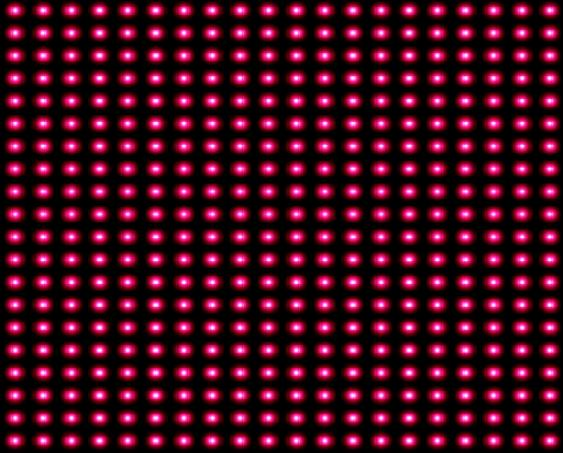
\includegraphics[width=0.48\textwidth]{./figures/shearoff.jpg}
\hspace{0.005cm}
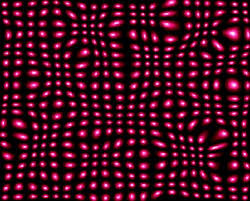
\includegraphics[width=0.48\textwidth]{./figures/shearon.jpg}\\
\vspace{1cm}
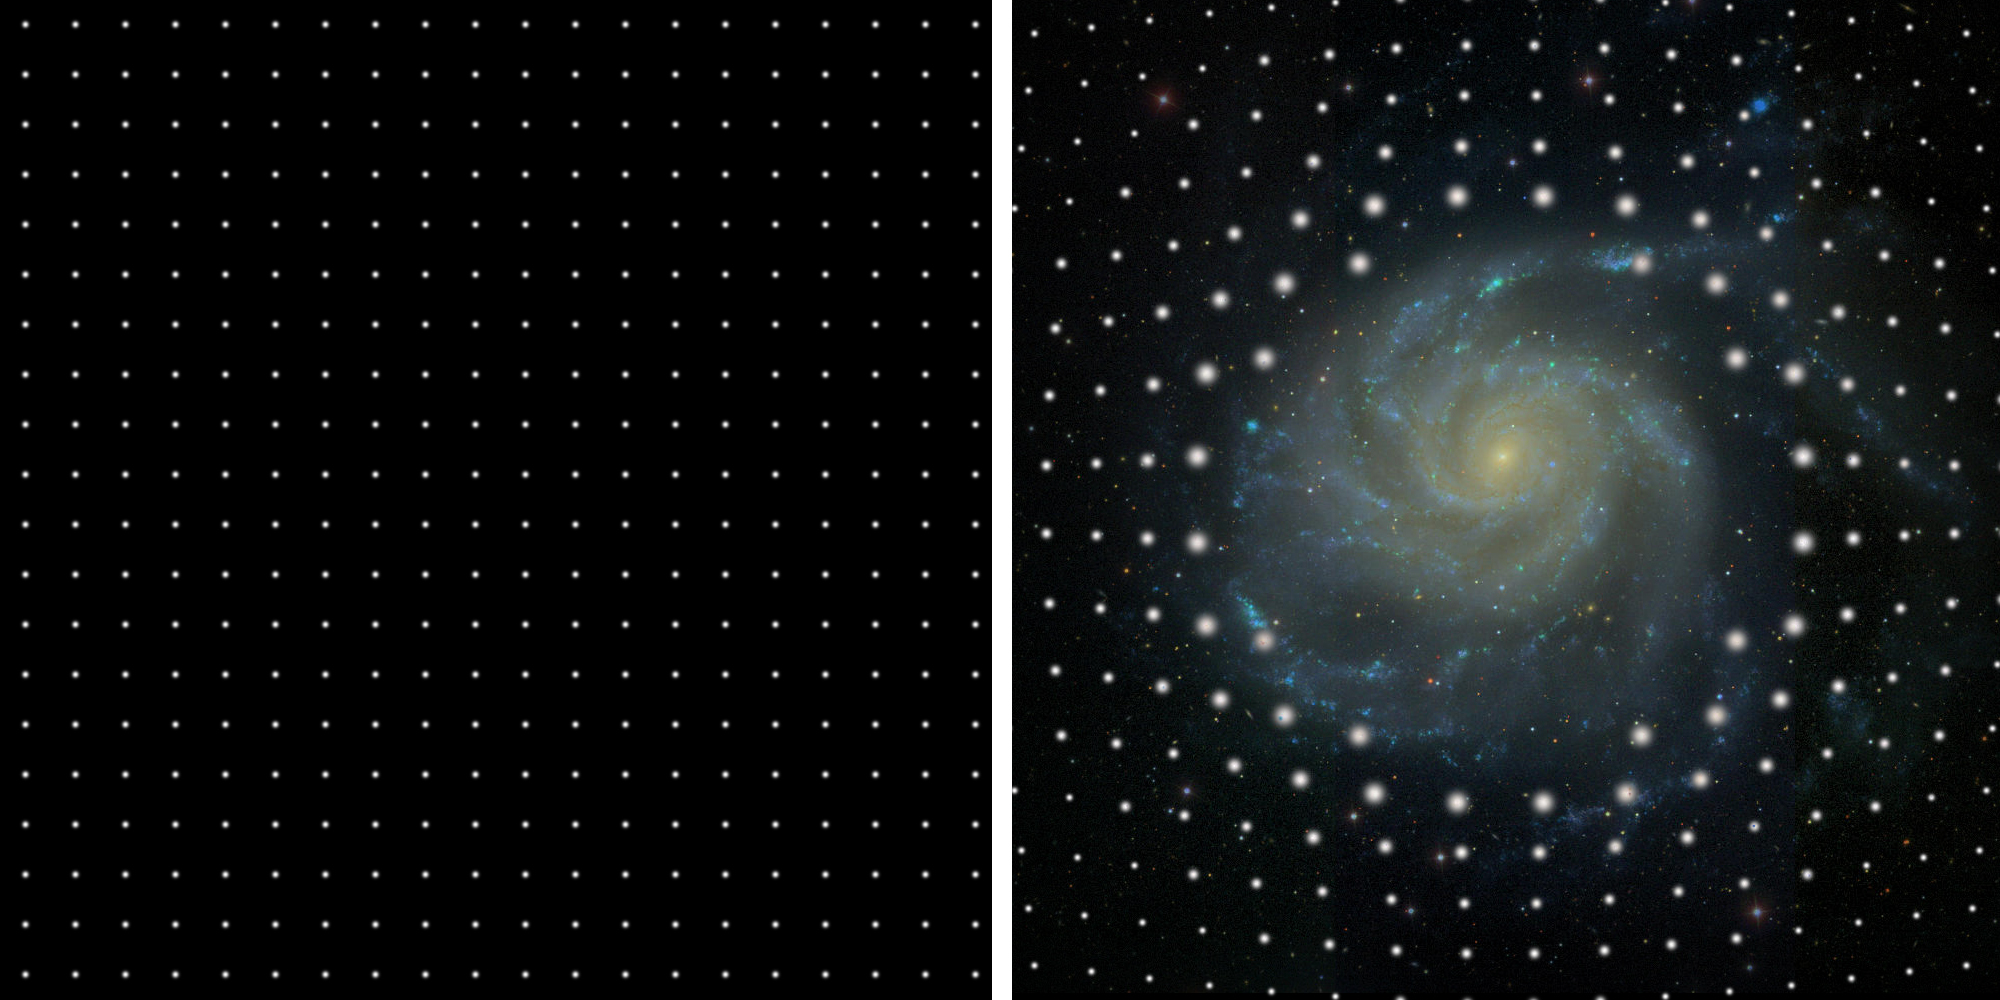
\includegraphics[width=0.98\textwidth]{./figures/numbercount.jpg}
\end{columns}
\end{frame}
%%%%%%%%%%%%%%%%%%%%%%%%%%%%%%%%%%%%%%%%%%%%%%%%%%%%%%%%%%%%%%%%%%%%%%%%%
\begin{frame}
\frametitle{\begin{small}\underline{{\bf Gravitational lensing.}}\end{small}}
Lensing map of an extended image:
$$\mathcal{I}(\vec\beta) = \mathcal{I}[\vec \beta(\vec\theta)] = \mathcal{I}[\vec\beta(\vec\theta_0)+\mathcal{J}\cdot(\vec\theta-\vec\theta_0)]$$
\vspace{0.1cm}
$$\mathcal{J} = \left(\begin{array}{ c c }
1-\kappa-\gamma_1 & -\gamma_2\\
\gamma_2 & 1-\kappa+\gamma_1\\
\end{array}\right)$$
\vspace{1cm}
\begin{columns}
\column{0.5\textwidth}
$\kappa\rightarrow$ convergence \\
$\gamma_1,\gamma_2\rightarrow$ shear
\column{0.5\textwidth}
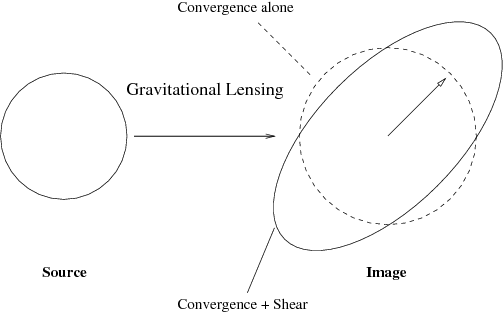
\includegraphics[width=\textwidth]{./figures/distortion.png}
\end{columns}
\end{frame}
%%%%%%%%%%%%%%%%%%%%%%%%%%%%%%%%%%%%%%%%%%%%%%%%%%%%%%%%%%%%%%%%%%%%%%%%%
\begin{frame}
\frametitle{\begin{small}\underline{{\bf Gravitational lensing.}}\end{small}}
$$
\mbox{Weak-lensing}
\left\{
\begin{array}{l}
\mbox{Shear}\\
\\
\\
\\
\mbox{\bf \color{red}Magnification}\left\{\begin{array}{l}\mbox{\bf \color{red}Number-count}\\ \\ \\ \mbox{Flux/magnitude}\\ \\ \\ \mbox{Size}\end{array}\right.
\end{array}\right.
$$
\end{frame}
%%%%%%%%%%%%%%%%%%%%%%%%%%%%%%%%%%%%%%%%%%%%%%%%%%%%%%%%%%%%%%%%%%%%%%%%%
\begin{frame}
\frametitle{\begin{small}\underline{{\bf Gravitational lensing.}}\end{small}}
\begin{columns}
\column{0.5\textwidth}
{\bf \underline{Magnification} }
$$\delta_\mu(\theta) = [\alpha(m)-1]2\kappa(\theta)$$
$$\kappa(\theta) = \frac{\Sigma(\theta)}{\Sigma_c}$$
\column{0.5\textwidth}
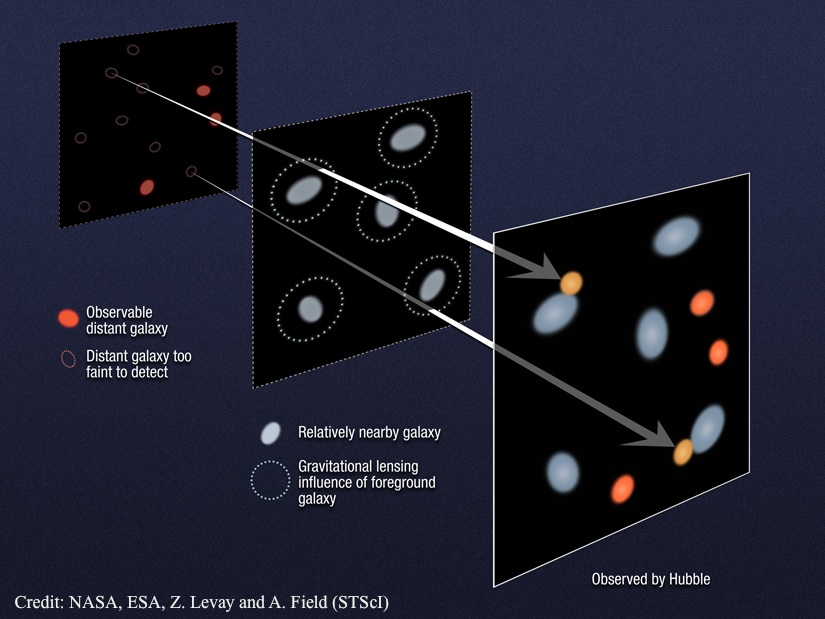
\includegraphics[width=\textwidth]{./figures/lenseffect.jpg}
\end{columns}
\begin{columns}
\column{0.5\textwidth}
{\bf \underline{gg-lensing} }
$$\langle\gamma_t\rangle(\theta) = \frac{\Delta\Sigma(\theta)}{\Sigma_c}$$
$$\Delta\Sigma(\theta) = \bar\Sigma(\theta'<\theta)-\Sigma(\theta)$$
\column{0.5\textwidth}
\vspace{0.1cm}
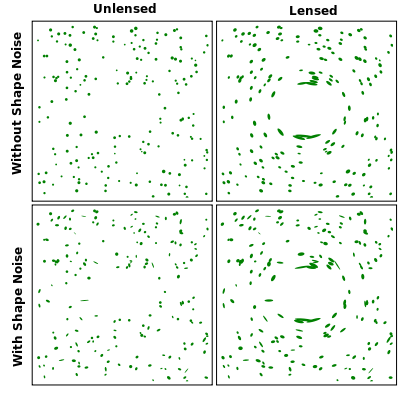
\includegraphics[width=\textwidth,trim={1cm 7cm 0cm 0.7cm},clip]{./figures/gglensing.png}
\end{columns}
\end{frame}
%%%%%%%%%%%%%%%%%%%%%%%%%%%%%%%%%%%%%%%%%%%%%%%%%%%%%%%%%%%%%%%%%%%%%%%%%
\begin{frame}
\frametitle{\begin{small}\underline{{\bf Gravitational lensing.}}\end{small}}
Probes of the underlying {\bf (dark-)matter field}.\\
\vspace{0.7cm}
Magnification \& shear {\bf complementary effects} of same phenomena.\\
\vspace{0.7cm}
{\bf Different systematic} effects:\\
\hspace{1cm}$\rightarrow$ gg-lensing: shape-related systematic.\\
\hspace{1cm}$\rightarrow$ magnification: redshift- \& completeness- related systematics.\\
\vspace{0.7cm}
Magnification has {\bf low S/N }.\\
\end{frame}
%%%%%%%%%%%%%%%%%%%%%%%%%%%%%%%%%%%%%%%%%%%%%%%%%%%%%%%%%%%%%%%%%%%%%%%%%
\begin{frame}
\frametitle{\begin{small}\underline{{\bf Gravitational lensing.}}\end{small}}
\begin{center}
{\bf \color{red} Why should we care about gravitational lensing?}
\vspace{0.5cm}
\begin{itemize}
\item Direct matter probe:\\
$\rightarrow$ No galaxy-bias assumption.\\
$\rightarrow$ No HOD modeling.\\
\vspace{0.5cm}
\item Different complementary probes of the same phenomena:\\
$\rightarrow$ {\bf Better control of systematic error.}
\end{itemize}
\end{center}
\end{frame}
%%%%%%%%%%%%%%%%%%%%%%%%%%%%%%%%%%%%%%%%%%%%%%%%%%%%%%%%%%%%%%%%%%%%%%%%%
\begin{frame}
\frametitle{\begin{small}\underline{{\bf Gravitational lensing.}}\end{small}}
\begin{center}
{\bf The KiDS-CFHTLens-DES conundrum.}\\
\vspace{0.5cm}
The intrinsic alignment:
\begin{itemize}
\item KiDS: $A_{IA}= +1.10, -1.17$.
\item DES: $A_{IA}=+0.5$.
\item CFHTLens: $A_{IA}=-3.6$.
\end{itemize}
\vspace{1cm}
{\bf \color{red}Magnification does not depend of the IA!}
\end{center}
\end{frame}
%%%%%%%%%%%%%%%%%%%%%%%%%%%%%%%%%%%%%%%%%%%%%%%%%%%%%%%%%%%%%%%%%%%%%%%%%
\begin{frame}[plain]
\begin{LARGE}
\begin{center}
{{\bf \color{blue}MAGNIFICATION DES-SV}}
\end{center}
\end{LARGE}
\end{frame}
%%%%%%%%%%%%%%%%%%%%%%%%%%%%%%%%%%%%%%%%%%%%%%%%%%%%%%%%%%%%%%%%%%%%%%%%%
\begin{frame}
\frametitle{\begin{small}\underline{{\bf Magnification DES-SV.}}\end{small}}
{\bf Traditional approach} to overcome low S/N \begin{footnotesize}(arXiv:1204.2830)\end{footnotesize}.
\vspace{0.5cm}
\begin{columns}
\column{0.5\textwidth}
Use Lyman Break Galaxies (LBGs):
\vspace{0.5cm}
\begin{itemize}
\item Steep $N(m) \rightarrow$ High $\alpha(m)$.
\item  $2 \lesssim z \lesssim 4$
\item Clean photo-z determination.
\item Downside: {\bf low density}.
\end{itemize}
\vspace{1cm}
\begin{center}
Only $10^4$ at DES-SV\\
$\Downarrow$\\
{\bf \color{red}Impossible the detection!}
\end{center}

\column{0.5\textwidth}
\begin{center}
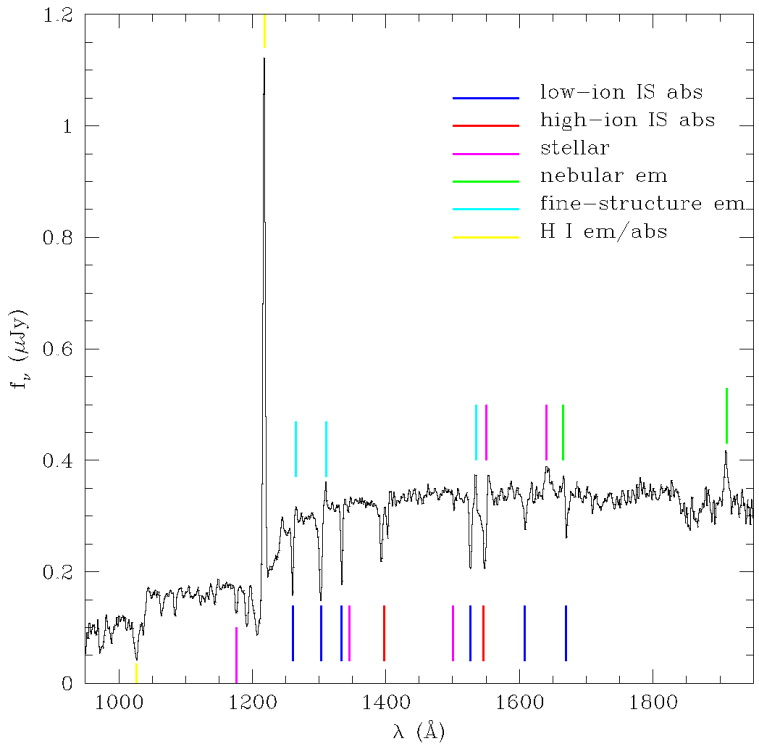
\includegraphics[width=\textwidth]{./figures/lbg_template.jpg}\\
\begin{footnotesize}(arXiv:astro-ph/0301230)\end{footnotesize}
\end{center}
\end{columns}
\end{frame}
%%%%%%%%%%%%%%%%%%%%%%%%%%%%%%%%%%%%%%%%%%%%%%%%%%%%%%%%%%%%%%%%%%%%%%%%%
\begin{frame}
\frametitle{\begin{small}\underline{{\bf Magnification DES-SV.}}\end{small}}
{\color{red}New approach!} Use all galaxies w/ hard photo-z cuts.\\
\begin{itemize}
\item Large density of galaxies.
\item Downside: need well controlled photo-z mixing.
\end{itemize}
\vspace{0.5cm}
Developed methodology with Dark Energy Survey SV-data.\\
$$A = 121\mbox{ deg}^2;\ \ \ \ \ \ N_l \sim 500000;\ \ \ \ \ \ N_s \sim 700000$$
\begin{center}
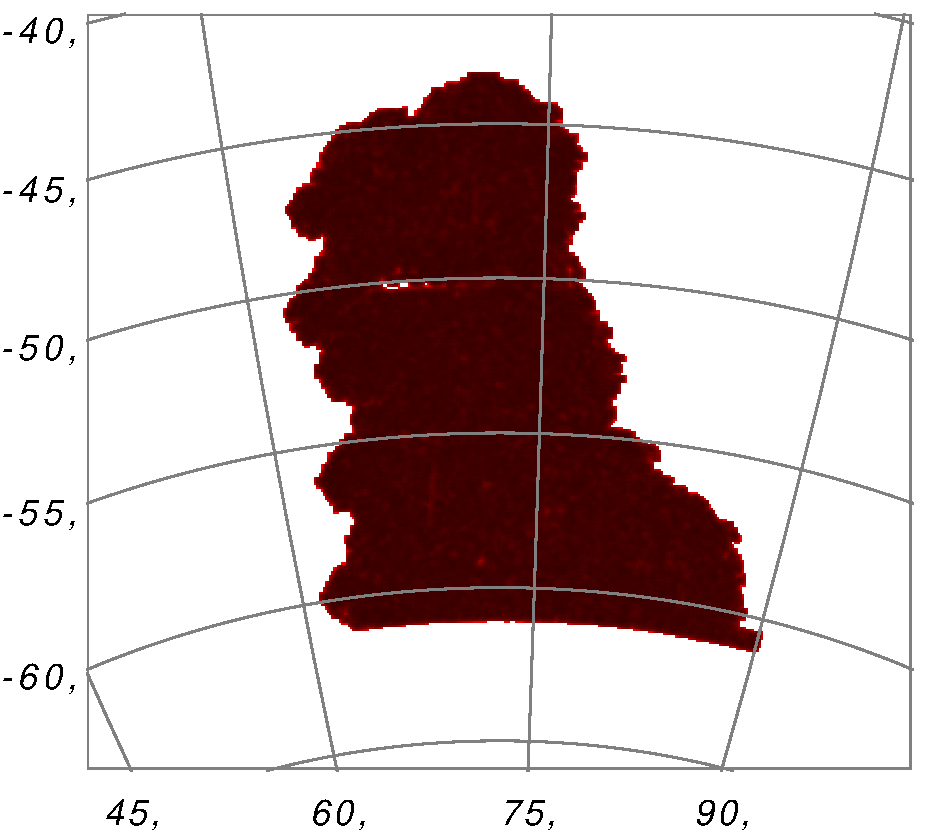
\includegraphics[height=0.36\textheight]{./figures/footprint.pdf}\hspace{0.5cm}
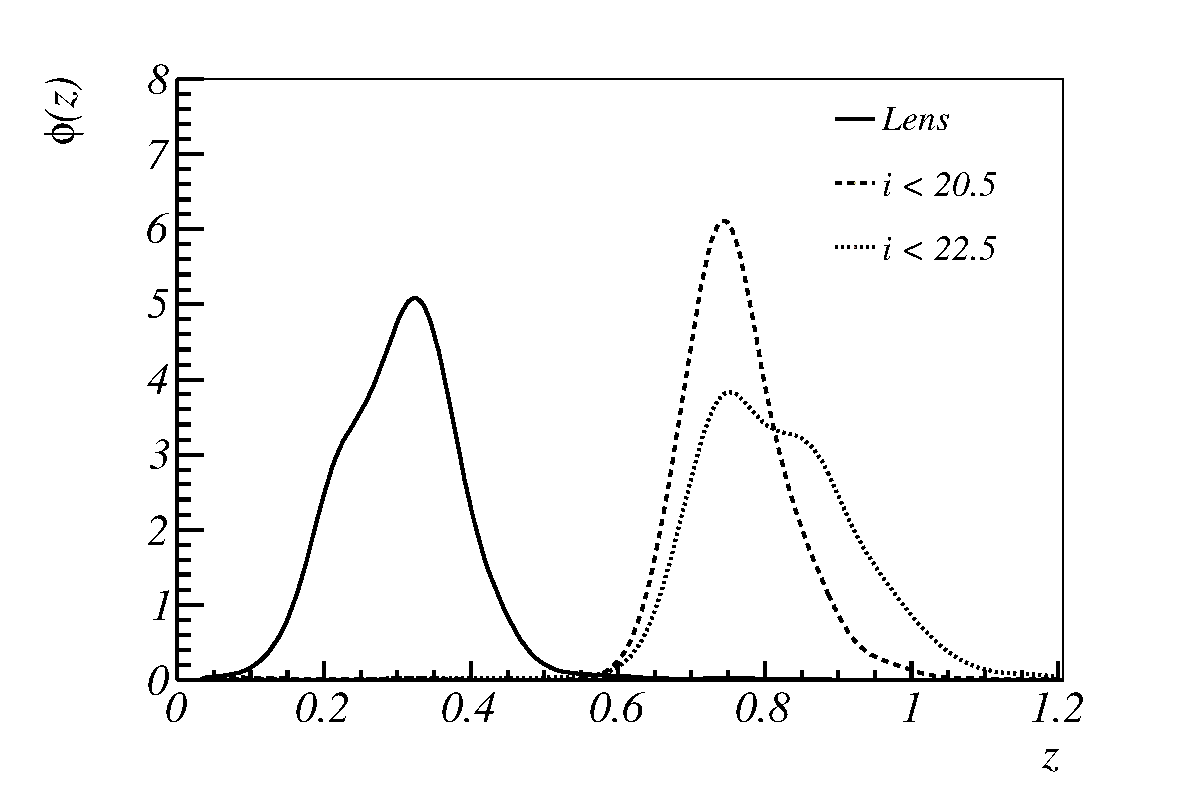
\includegraphics[height=0.4\textheight]{./figures/TPZ_phis_i.pdf}\\
\end{center}
\begin{footnotesize}({\tt des.ncsa.illinois.edu/releases/SVA1})\end{footnotesize}
\end{frame}
%%%%%%%%%%%%%%%%%%%%%%%%%%%%%%%%%%%%%%%%%%%%%%%%%%%%%%%%%%%%%%%%%%%%%%%%%
\begin{frame}
\frametitle{\begin{small}\underline{{\bf Magnification DES-SV.}}\end{small}}
{\bf The data sample:} DES-SV-Gold.\\
\vspace{0.2cm}
\begin{itemize}
\item S/G-separation: {\tt modest\_class}.
\vspace{0.2cm}
\item Depth: $r_{lim}> 23.0$ \& $i_{lim}> 22.5$ \& $z_{lim}>22.0$.
\vspace{0.2cm}
\item Mask: worst 4\% \& bright-star halos removed.
\vspace{0.2cm}
\item Edges: $r_{fracdet}=1$ \& $i_{fracdet}=1$ \& $z_{fracdet}=1$.
\vspace{0.2cm}
\item Uniformity: $r<23.0$ \& $i<22.5$ \& $z<22.0$.\\
$\rightarrow$ Also improves the S/G separation.\\
$\rightarrow$ Compatibility with Crocce et al. 2015 benchmark sample.
\vspace{0.2cm}
\item `Crazy colors' removed.
\end{itemize}
\end{frame}
%%%%%%%%%%%%%%%%%%%%%%%%%%%%%%%%%%%%%%%%%%%%%%%%%%%%%%%%%%%%%%%%%%%%%%%%%
\begin{frame}
\frametitle{\begin{small}\underline{{\bf Magnification DES-SV.}}\end{small}}
{\bf The measurement of number-count magnification:}\\
\begin{enumerate}[1]
\item Divide lens \& source sample.
\item Divide magnitude sub-samples: trace the number-count slope.
$$\alpha(m) = \frac{d}{dm}[N(m)]$$
\item Cross-correlate samples Landy-Szalay estimator:
$$\omega_{LS}(\theta) = \frac{D_LD_S-D_LR_S-D_SR_L+R_LR_S}{R_LR_S}$$
\end{enumerate}
\end{frame}
%%%%%%%%%%%%%%%%%%%%%%%%%%%%%%%%%%%%%%%%%%%%%%%%%%%%%%%%%%%%%%%%%%%%%%%%%
\begin{frame}
\frametitle{\begin{small}\underline{{\bf Magnification DES-SV.}}\end{small}}
{\bf Lens:}\\
$\rightarrow$ $0.2 < z_{TPZ} < 0.4$ \& $i<22.5$.\\
\vspace{0.5cm}
{\bf Sources:}\\
$\rightarrow$ $0.7 < z_{TPZ} < 1.0$.\\
\vspace{0.2cm}
Five subsamples {\bf \color{red}nested} within each band:\\
\vspace{0.2cm}
\begin{itemize}
\item R: $r<21.0$; $r<21.5$; $r<22.0$; $r<22.5$; $r<23.0$.
\vspace{0.2cm}
\item I: $i<20.5$; $i<21.0$; $i<21.5$; $i<22.0$; $i<22.5$.
\vspace{0.2cm}
\item Z: $z<20.0$; $z<20.5$; $z<21.0$; $z<21.5$; $z<22.0$.
\end{itemize}
\begin{center}
{\bf To trace the evolution of the number-count slope parameter.}
\end{center}
\end{frame}
%%%%%%%%%%%%%%%%%%%%%%%%%%%%%%%%%%%%%%%%%%%%%%%%%%%%%%%%%%%%%%%%%%%%%%%%%
\begin{frame}
\frametitle{\begin{small}\underline{{\bf Magnification DES-SV.}}\end{small}}
\begin{center}
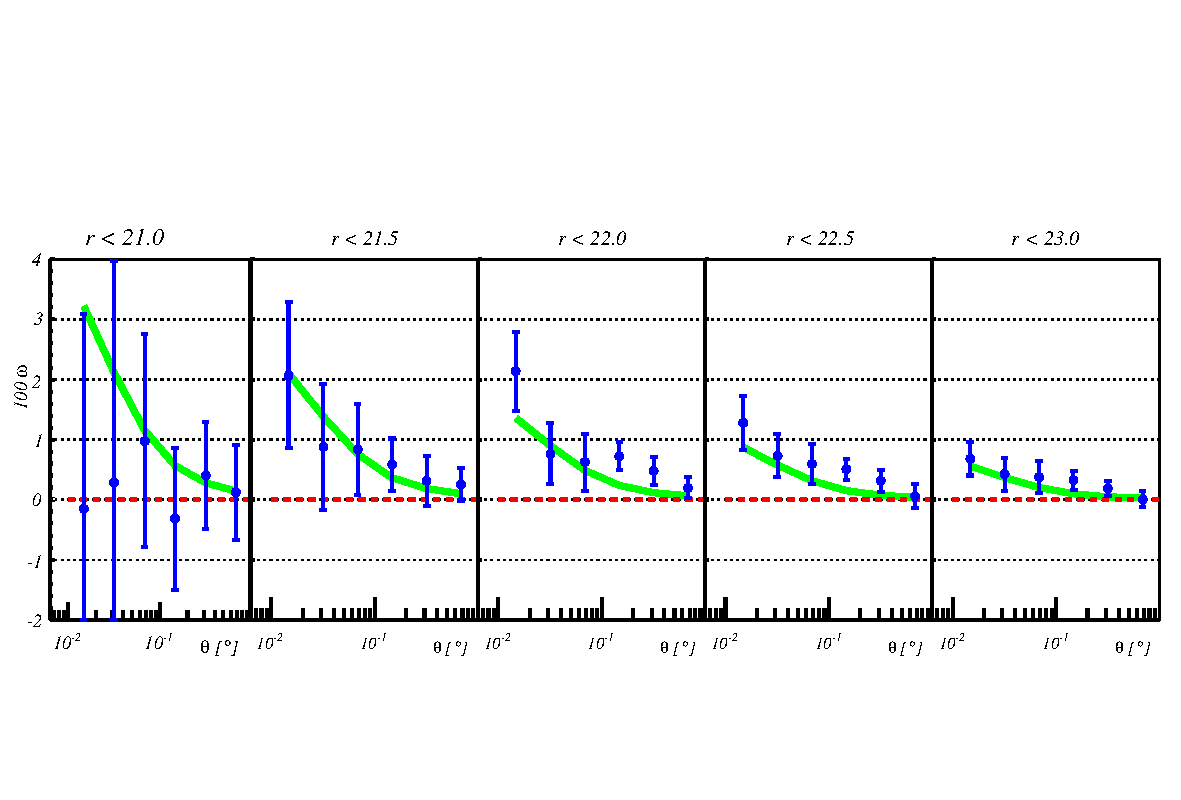
\includegraphics[width=\textwidth,trim={0 2.3cm 0 3.5cm},clip]{./figures/mag_r.pdf}
\end{center}
\begin{footnotesize}(arXiv:1611.10326)\end{footnotesize}
\end{frame}
%%%%%%%%%%%%%%%%%%%%%%%%%%%%%%%%%%%%%%%%%%%%%%%%%%%%%%%%%%%%%%%%%%%%%%%%%
\begin{frame}
\frametitle{\begin{small}\underline{{\bf Magnification DES-SV.}}\end{small}}
\begin{center}
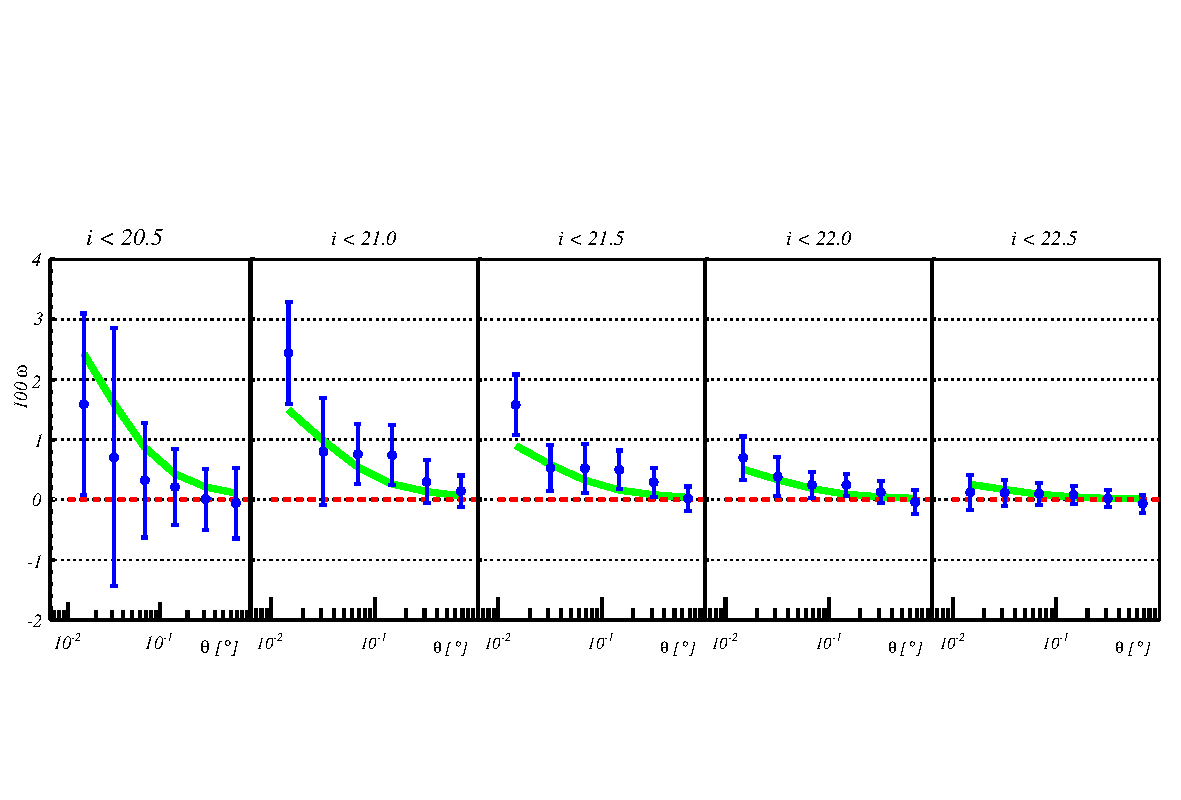
\includegraphics[width=\textwidth,trim={0 2.3cm 0 3.5cm},clip]{./figures/mag_i.pdf}
\end{center}
\begin{footnotesize}(arXiv:1611.10326)\end{footnotesize}
\end{frame}
%%%%%%%%%%%%%%%%%%%%%%%%%%%%%%%%%%%%%%%%%%%%%%%%%%%%%%%%%%%%%%%%%%%%%%%%%
\begin{frame}
\frametitle{\begin{small}\underline{{\bf Magnification DES-SV.}}\end{small}}
\begin{center}
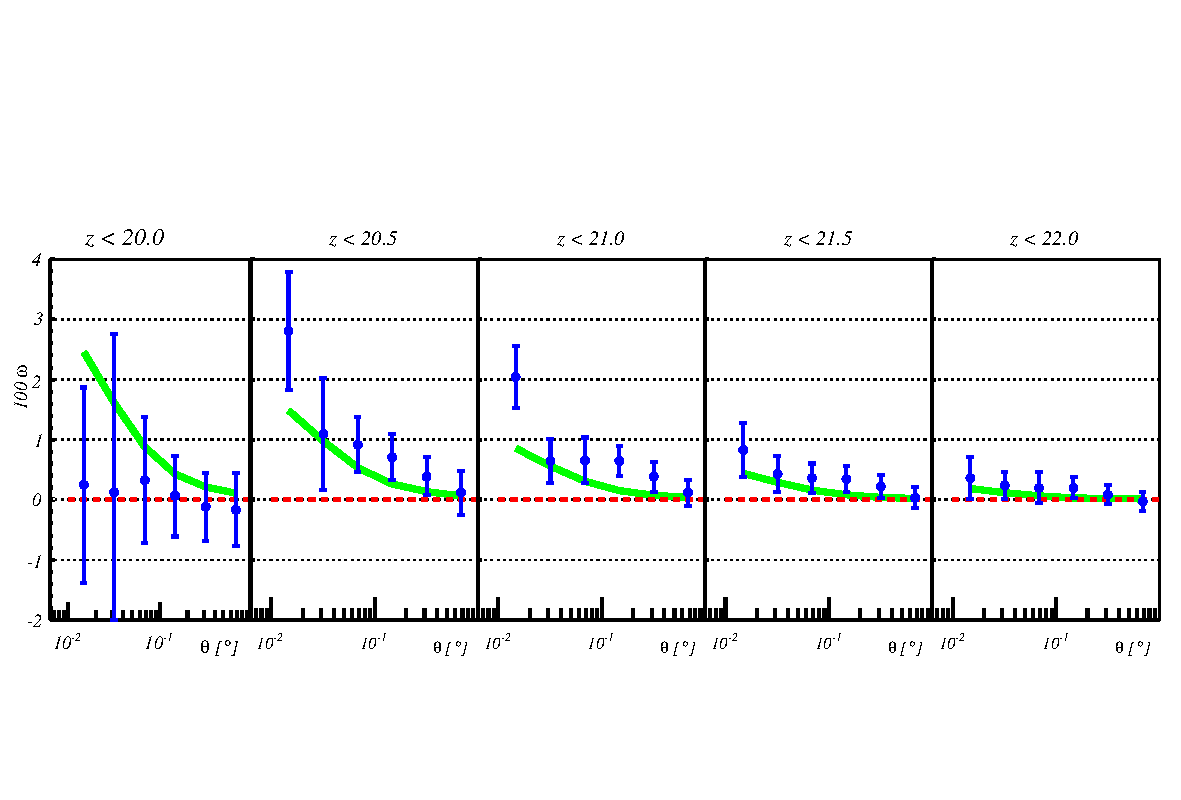
\includegraphics[width=\textwidth,trim={0 2.3cm 0 3.5cm},clip]{./figures/mag_z.pdf}
\end{center}
\begin{footnotesize}(arXiv:1611.10326)\end{footnotesize}
\end{frame}
%%%%%%%%%%%%%%%%%%%%%%%%%%%%%%%%%%%%%%%%%%%%%%%%%%%%%%%%%%%%%%%%%%%%%%%%%
\begin{frame}
\frametitle{\begin{small}\underline{{\bf Magnification DES-SV.}}\end{small}}
{\bf Theoretical calculations:}
$$\omega(\theta) = b_L[\alpha(m)-1]2\kappa(\theta)$$
\begin{itemize}
\item $\kappa$ from weak-lensing theory.
\vspace{0.2cm}
\item Assume a $\Lambda$CDM Universe with Planck 2015 parameters.
\vspace{0.2cm}
\item Linear, constant, redshift independent bias from Crocce et al. 2015.
\end{itemize}
\end{frame}
%%%%%%%%%%%%%%%%%%%%%%%%%%%%%%%%%%%%%%%%%%%%%%%%%%%%%%%%%%%%%%%%%%%%%%%%%
\begin{frame}
\frametitle{\begin{small}\underline{{\bf Magnification DES-SV.}}\end{small}}
\begin{itemize}
\item $\alpha$ Fit N(m) to Schechter function and do derivative (analytical).
$$N_\mu(m) = A\left[10^{0.4(m-m_*)}\right]^\beta\times\exp\left[-10^{0.4(m-m*)}\right]$$
\end{itemize}
\vspace{0.2cm}
\begin{center}
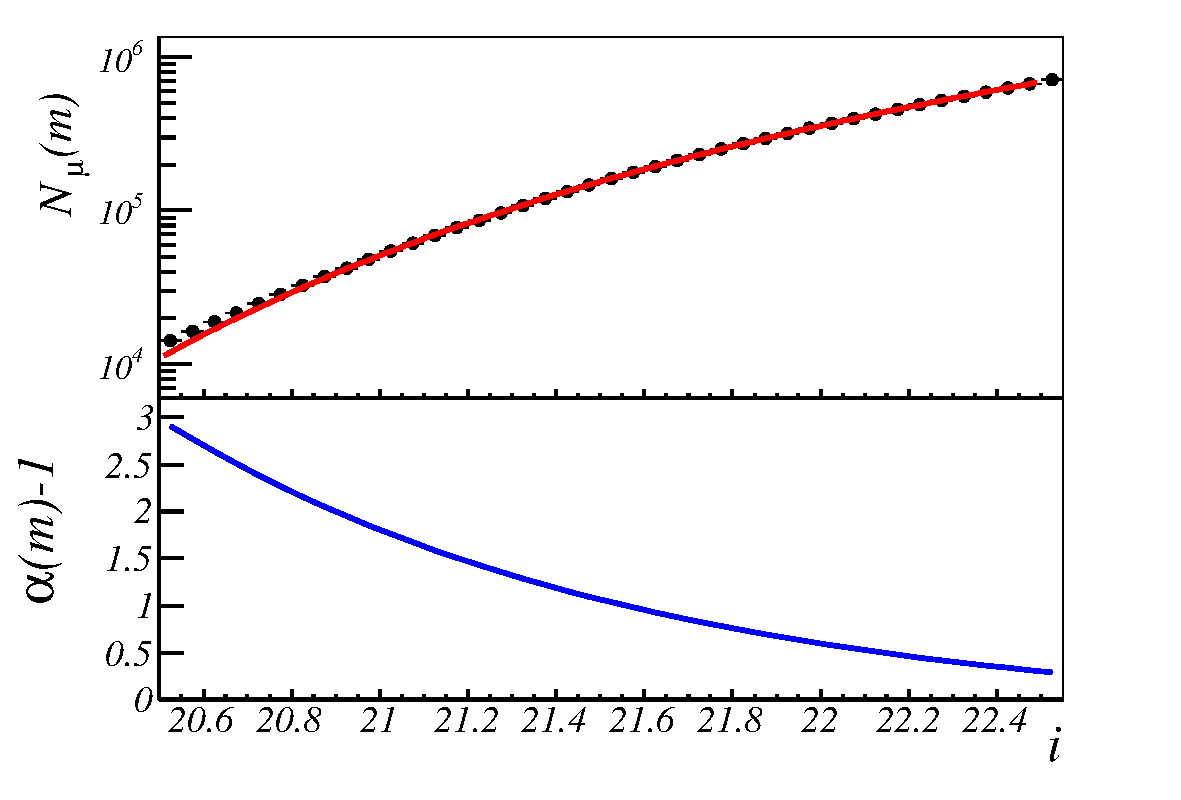
\includegraphics[width=0.6\textwidth]{./alphai.pdf}
\end{center}
\end{frame}
%%%%%%%%%%%%%%%%%%%%%%%%%%%%%%%%%%%%%%%%%%%%%%%%%%%%%%%%%%%%%%%%%%%%%%%%%
\begin{frame}
\frametitle{\begin{small}\underline{{\bf Magnification DES-SV.}}\end{small}}
{\bf Compatibility with theory:}\\
\begin{center}
$\chi^2_{\rm Planck} =\sum\limits_{\eta\nu ij}[\tilde \omega_{\rm LS_i}(\theta_\eta)-\omega_{\rm LS_i}(\theta_\eta)]$\\
$C^{-1}(\omega_{\rm LS_i}(\theta_\eta);\omega_{\rm LS_j}(\theta_\nu))[\tilde \omega_{\rm LS_j}(\theta_\nu)-\omega_{\rm LS_j}(\theta_\nu)]$\\
\vspace{1cm}
$\chi^2_{\rm zero} =\sum\limits_{\eta\nu ij}\tilde \omega_{\rm LS_i}(\theta_\eta)C^{-1}(\omega_{\rm LS_i}(\theta_\eta);\omega_{\rm LS_j}(\theta_\nu))\tilde \omega_{\rm LS_j}(\theta_\nu)$\\
\end{center}
{\bf Significance of the detection:}\\
\begin{center}
$\mathcal{B} = \frac{P(M|\Theta)}{P(Z|\Theta)}\frac{P(M)}{P(Z)}$\\
\vspace{0.5cm}
$P(M|\Theta) = e^{-\chi^2_{Planck}/2}; P(Z|\Theta) = e^{-\chi^2_{zero}/2}$\\
\vspace{0.5cm}
$P(M) = P(Z)$
\end{center}
\end{frame}
%%%%%%%%%%%%%%%%%%%%%%%%%%%%%%%%%%%%%%%%%%%%%%%%%%%%%%%%%%%%%%%%%%%%%%%%%
\begin{frame}
\frametitle{\begin{small}\underline{{\bf Magnification DES-SV.}}\end{small}}
{\bf Covariance matrix:}\\
\begin{center}
$C_{\rm S}(\omega_{\rm LS_i}(\theta_\eta);\omega_{\rm LS_j}(\theta_\nu)) = \frac{N_{\rm JK}}{N_{\rm JK}-1}$
$\times \sum\limits_k^{N_{\rm JK}}[\omega_{\rm LS_i}^k(\theta_\eta)-\omega_{\rm LS_i}(\theta_\eta)][\omega_{\rm LS_j}^k(\theta_\nu)-\omega_{\rm LS_j}(\theta_\nu)]\nonumber$
\begin{columns}
\column{0.5\textwidth}
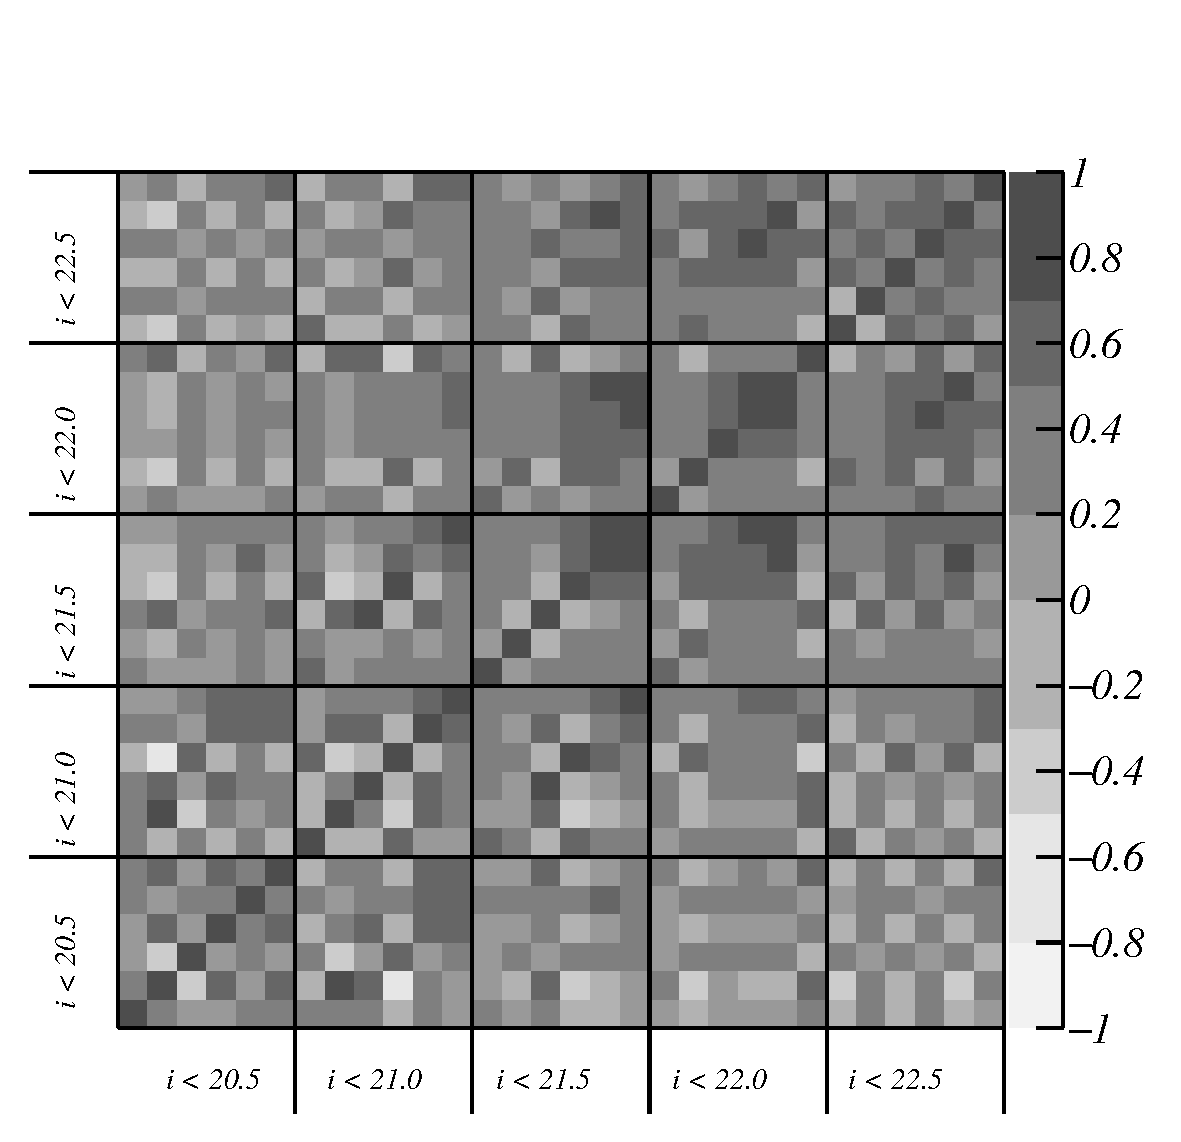
\includegraphics[width=\textwidth]{./cov_matrix_mag_auto_i.pdf}
\column{0.5\textwidth}
$$N_{JK}=120$$
\end{columns}
\end{center}
\end{frame}
%%%%%%%%%%%%%%%%%%%%%%%%%%%%%%%%%%%%%%%%%%%%%%%%%%%%%%%%%%%%%%%%%%%%%%%%%
\begin{frame}
\frametitle{\begin{small}\underline{{\bf Magnification DES-SV.}}\end{small}}
\begin{center}
\begin{table}
\begin{center}\adjustbox{max width=0.5\textwidth}{\begin{tabular}{ c | c c | c c }
Sample & $\log_{10}\mathcal{B}$ & $\chi^2/ndof$  & $\log_{10}\mathcal{B}$ & $\chi^2/ndof$ \\
\hline
$r<21.0$ &-0.3 & 1.9/6 & & \\
$r<21.5$ & 0.8 & 0.8/6 & & \\
$r<22.0$ & 2.0 & 6.6/6 & {\bf \color{red}3.9} & {\bf 21.6/30}\\
$r<22.5$ & 2.3 & 7.0/6 & & \\
$r<23.0$ & 1.1 & 4.2/6 & & \\
 \hline
$i<20.5$ & 0.2 & 0.9/6 & & \\
$i<21.0$ & 2.1 & 2.0/6 & & \\
$i<21.5$ & 2.5 & 4.5/6 & {\bf \color{red}3.5} & {\bf 24.2/30}\\
$i<22.0$ & 1.0 & 1.7/6 & & \\
$i<22.5$ & 0.0 & 1.5/6 & & \\
 \hline
$z<20.0$ & -0.4& 2.6/6 & & \\
$z<20.5$ & 2.3 & 2.6/6 & & \\
$z<21.0$ & 2.6 & 8.8/6 & {\bf \color{red}3.9} & {\bf 37.9/30}\\
$z<21.5$ & 0.9 & 3.5/6 & & \\
$z<22.0$ & 0.5 & 2.1/6 & & \\

\end{tabular} }\end{center}
\end{table}
\vspace{1cm}
{\bf \color{red} Magnification has been detected!}
\end{center}
\end{frame}
%%%%%%%%%%%%%%%%%%%%%%%%%%%%%%%%%%%%%%%%%%%%%%%%%%%%%%%%%%%%%%%%%%%%%%%%%
\begin{frame}
\frametitle{\begin{small}\underline{{\bf Magnification DES-SV.}}\end{small}}
{\bf Systematic analysis:}\\
\begin{itemize}
\item Stellar contamination.
\vspace{0.2cm}
\item Number-count slope determination.
\vspace{0.2cm}
\item Dust extinction.
\end{itemize}
\begin{center}
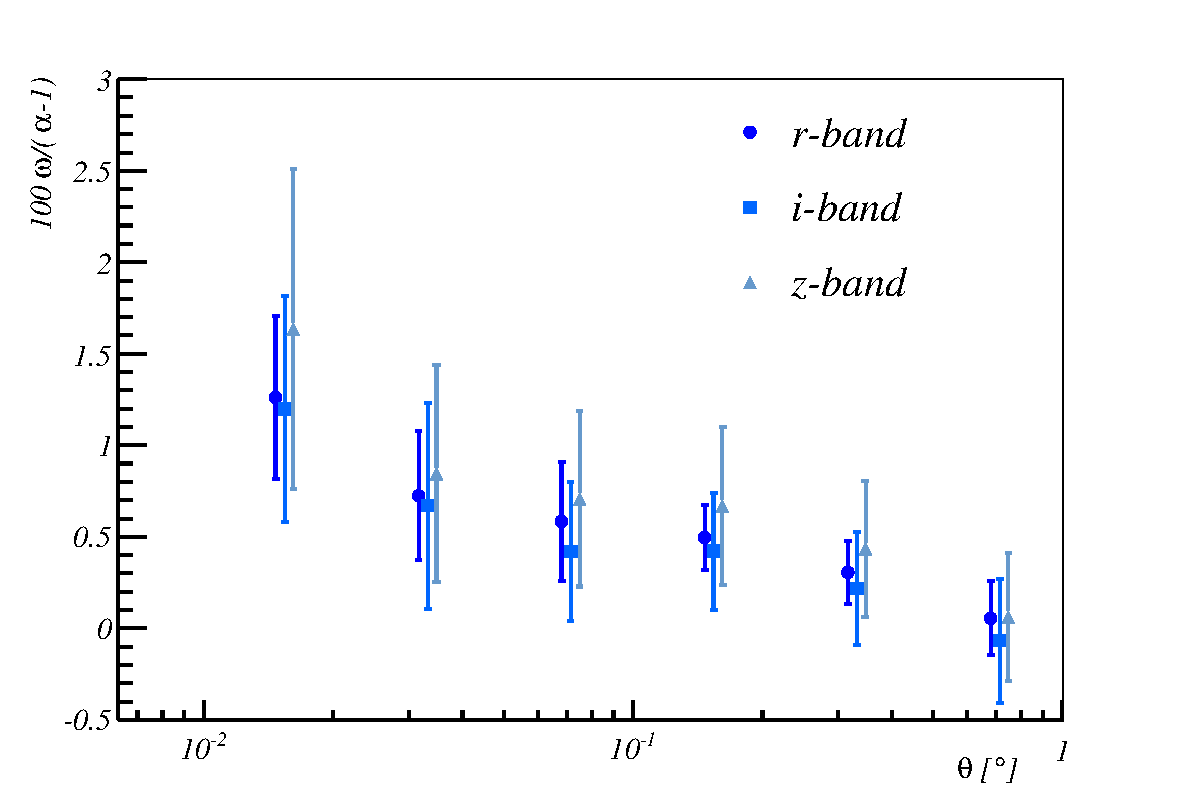
\includegraphics[width=0.6\textwidth]{./acromatic_short.pdf}\\
{\bf \color{red}None of them had a relevant impact. }
\end{center}
\end{frame}
%%%%%%%%%%%%%%%%%%%%%%%%%%%%%%%%%%%%%%%%%%%%%%%%%%%%%%%%%%%%%%%%%%%%%%%%%
\begin{frame}
\frametitle{\begin{small}\underline{{\bf Magnification DES-SV.}}\end{small}}
{\bf Survey observing conditions.}
\begin{itemize}
\item Uniform depth allows uniform randoms.
\vspace{0.2cm}
\item Used the {\scshape Balrog} simulations:\\ ({\tt https://github.com/emhuff/Balrog})
\begin{enumerate}[1]
\item Synthetic images of galaxies are generated.
\vspace{0.2cm}
\item Images are convolved with measured PSF.
\vspace{0.2cm}
\item Individual images injected into real DES images.
\vspace{0.2cm}
\item Real + simulated go though the whole pipeline.
\vspace{0.2cm}
\end{enumerate}
\end{itemize}
\end{frame}
%%%%%%%%%%%%%%%%%%%%%%%%%%%%%%%%%%%%%%%%%%%%%%%%%%%%%%%%%%%%%%%%%%%%%%%%%
\begin{frame}
\frametitle{\begin{small}\underline{{\bf Magnification DES-SV.}}\end{small}}
{\bf\scshape Balrog:}
\begin{itemize}
\item Map {\it real} $\rightarrow$ {\it observed} quantities.
\vspace{0.2cm}
\item {\bf \color{red} Determines the window function of the survey.}
\vspace{0.2cm}
\item Measures the completeness, depth, uniformity...
\vspace{0.2cm}
\item Takes into account un-blending.
\end{itemize}
\begin{center}
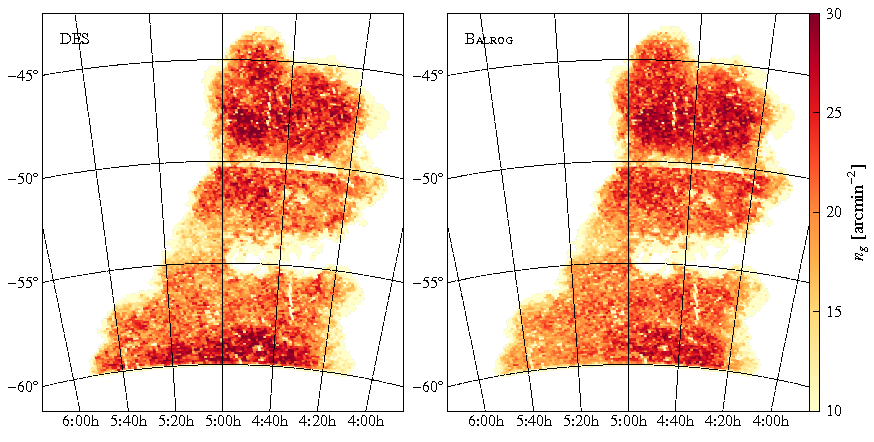
\includegraphics[width=0.6\textwidth]{./balrog_footprint.png}
\end{center}
\end{frame}
%%%%%%%%%%%%%%%%%%%%%%%%%%%%%%%%%%%%%%%%%%%%%%%%%%%%%%%%%%%%%%%%%%%%%%%%%
\begin{frame}
\frametitle{\begin{small}\underline{{\bf Magnification DES-SV.}}\end{small}}
\begin{itemize}
\item First time {\scshape Balrog} is used for a science measurement.
\vspace{0.2cm}
\item Provides reliable and un-biased way to deal with systematic.
\vspace{0.2cm}
\item {\bf Downside:} as good as your input catalog.
$\rightarrow$ COSMOS is enough for DES image-quality.
\end{itemize}
\vspace{0.2cm}
\begin{center}
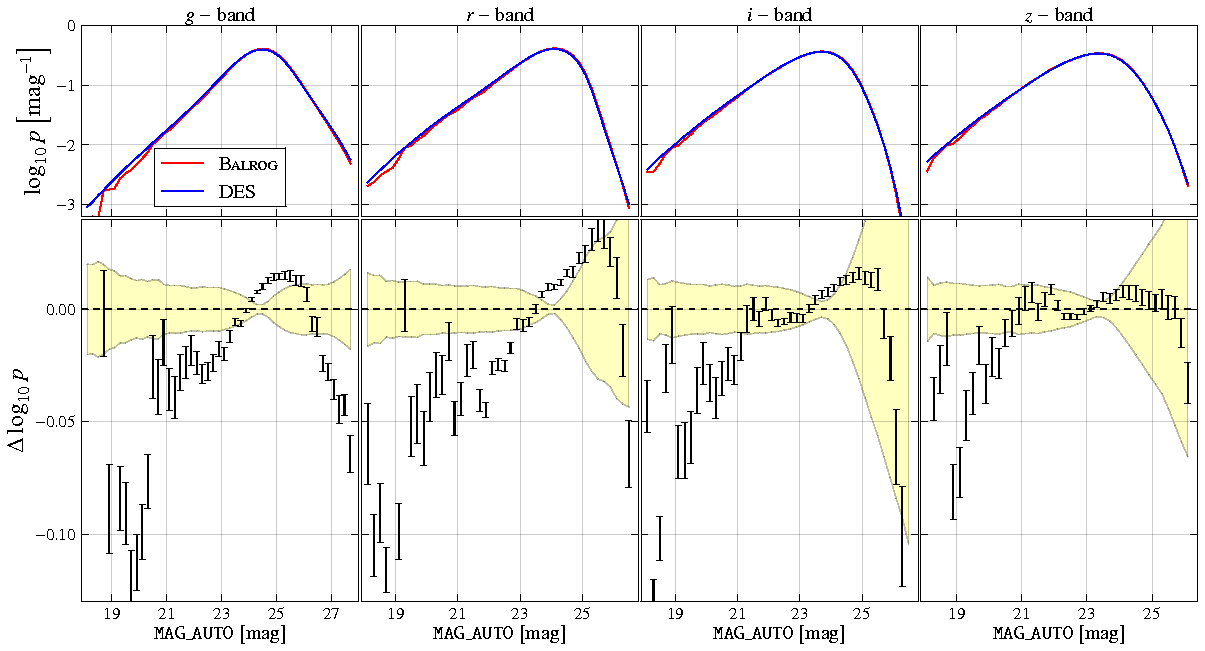
\includegraphics[width=0.7\textwidth,trim={0 0 0 0},clip]{./magdist_balrog.png}
\end{center}
\end{frame}
%%%%%%%%%%%%%%%%%%%%%%%%%%%%%%%%%%%%%%%%%%%%%%%%%%%%%%%%%%%%%%%%%%%%%%%%%
\begin{frame}
\frametitle{\begin{small}\underline{{\bf Magnification DES-SV.}}\end{small}}
{\bf Photo-z contamination:} Theoretical expected contamination.
\begin{center}
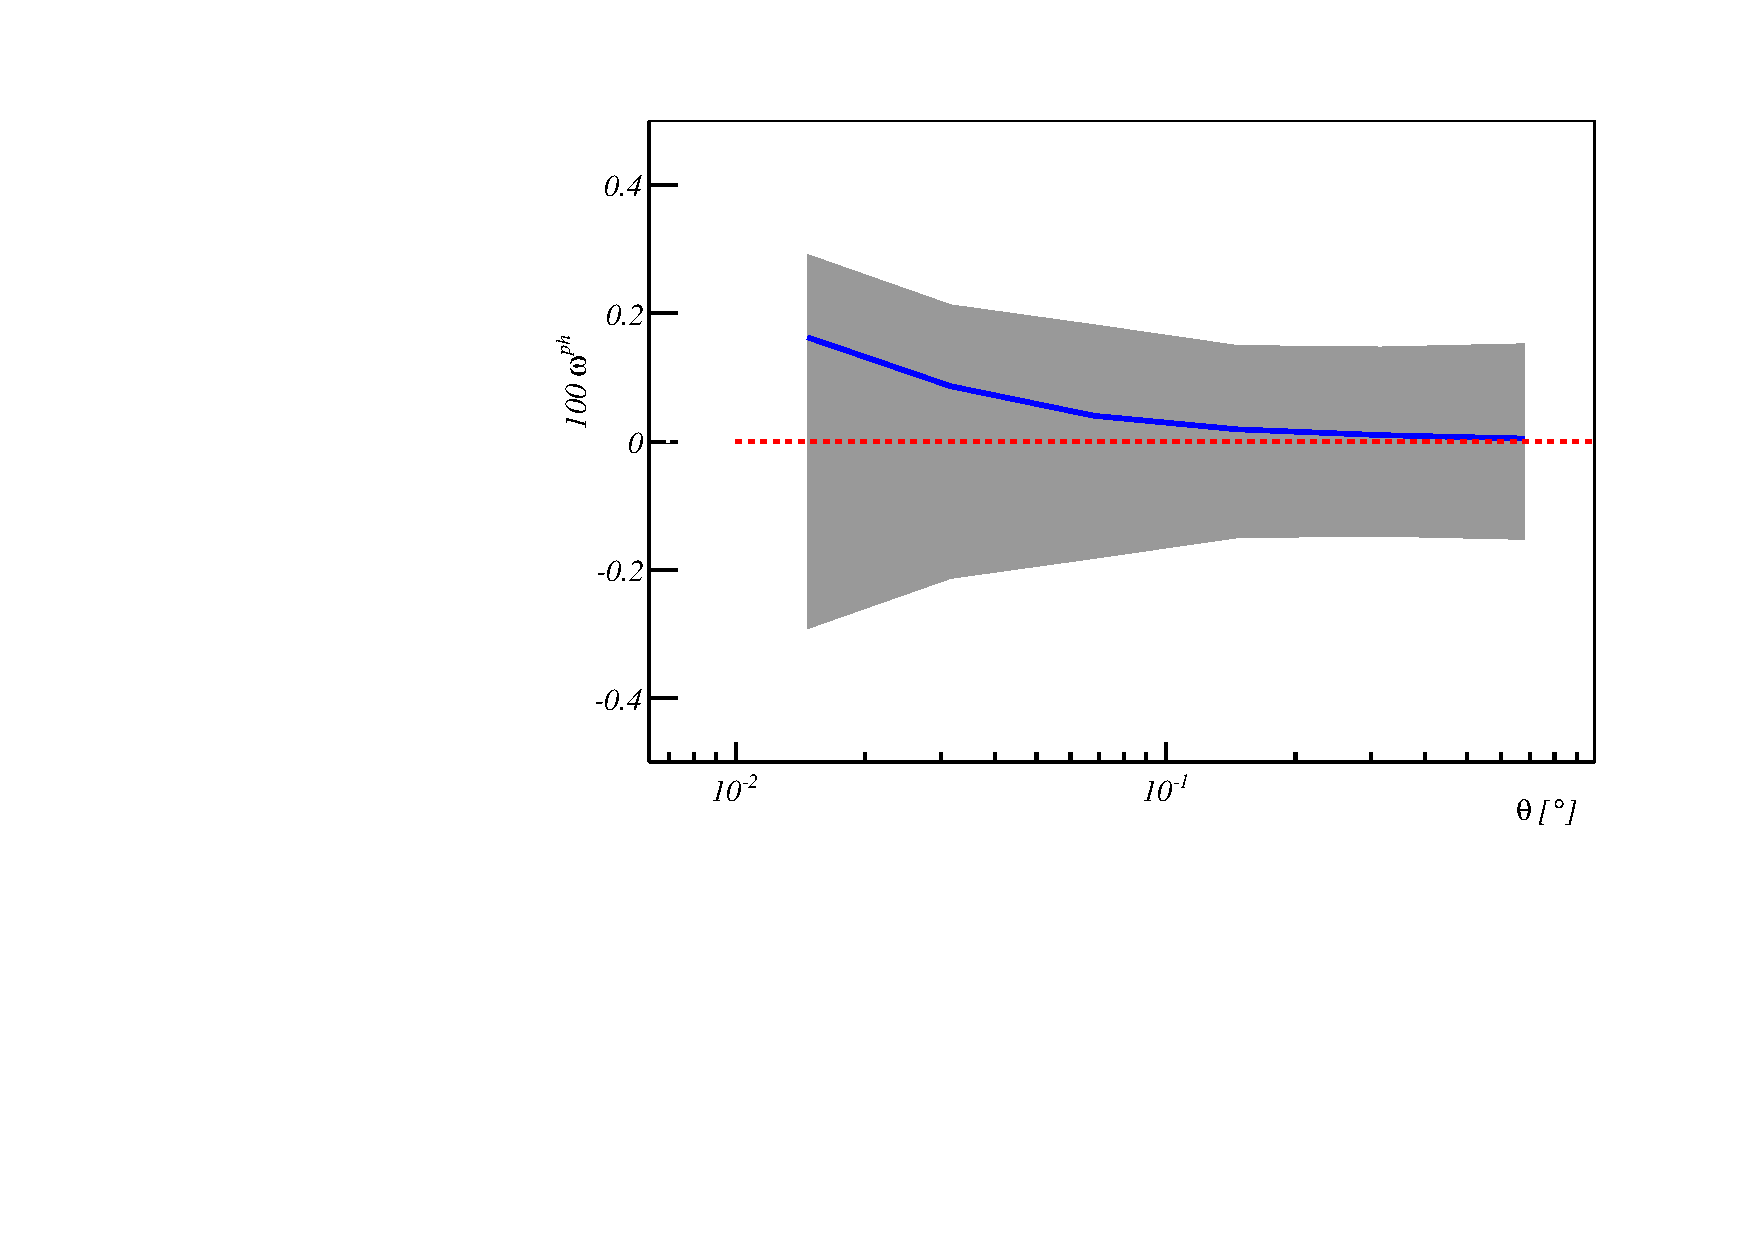
\includegraphics[width=0.75\textwidth]{./mag_itheo_photoz_short.pdf}
\end{center}
\end{frame}
%%%%%%%%%%%%%%%%%%%%%%%%%%%%%%%%%%%%%%%%%%%%%%%%%%%%%%%%%%%%%%%%%%%%%%%%%
\begin{frame}
\frametitle{\begin{small}\underline{{\bf Magnification DES-SV.}}\end{small}}
{\bf Photo-z contamination:} Simulated contamination.
\begin{center}
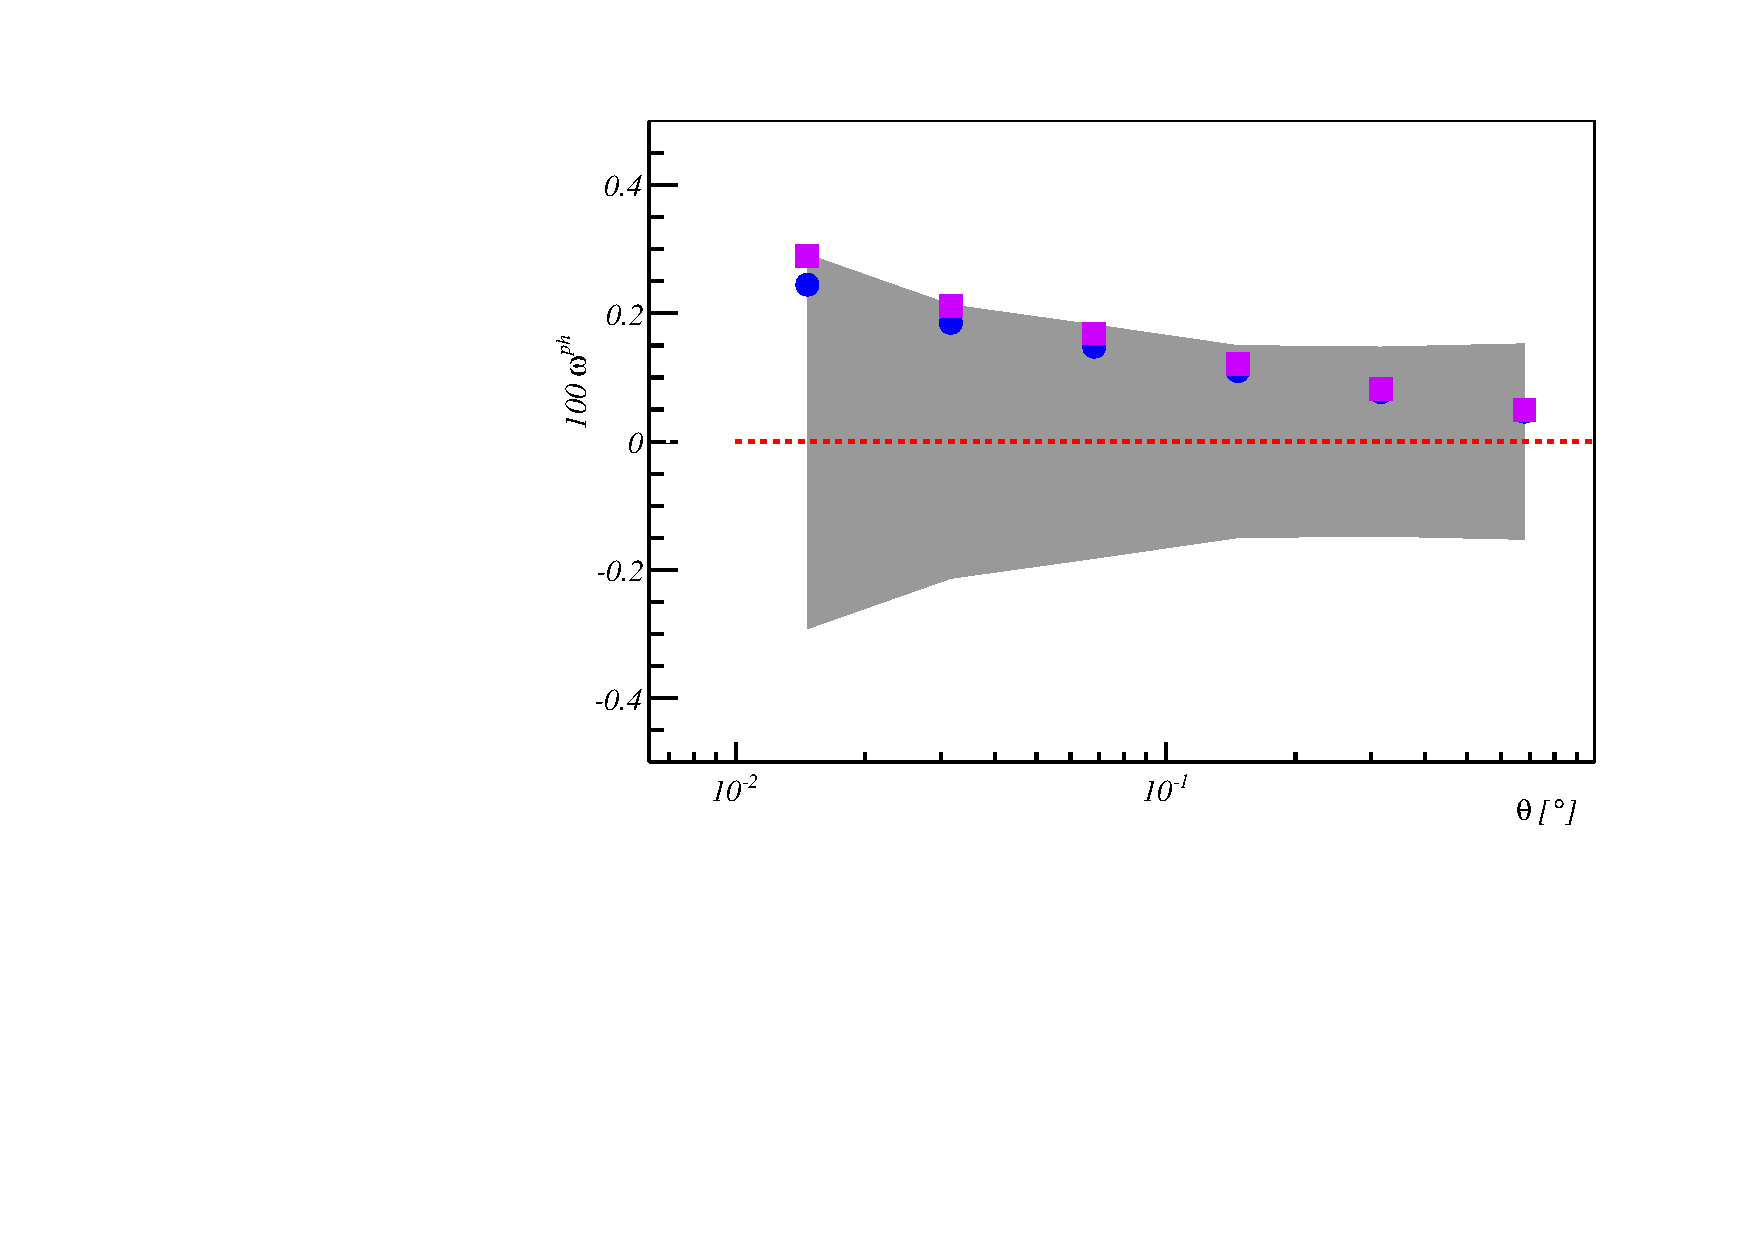
\includegraphics[width=0.75\textwidth]{./mag_i_mix_short.pdf}
\end{center}
\end{frame}
%%%%%%%%%%%%%%%%%%%%%%%%%%%%%%%%%%%%%%%%%%%%%%%%%%%%%%%%%%%%%%%%%%%%%%%%%
\begin{frame}
\frametitle{\begin{small}\underline{{\bf Magnification DES-SV.}}\end{small}}
{\bf Photo-z contamination:} Code comparison.
\begin{center}
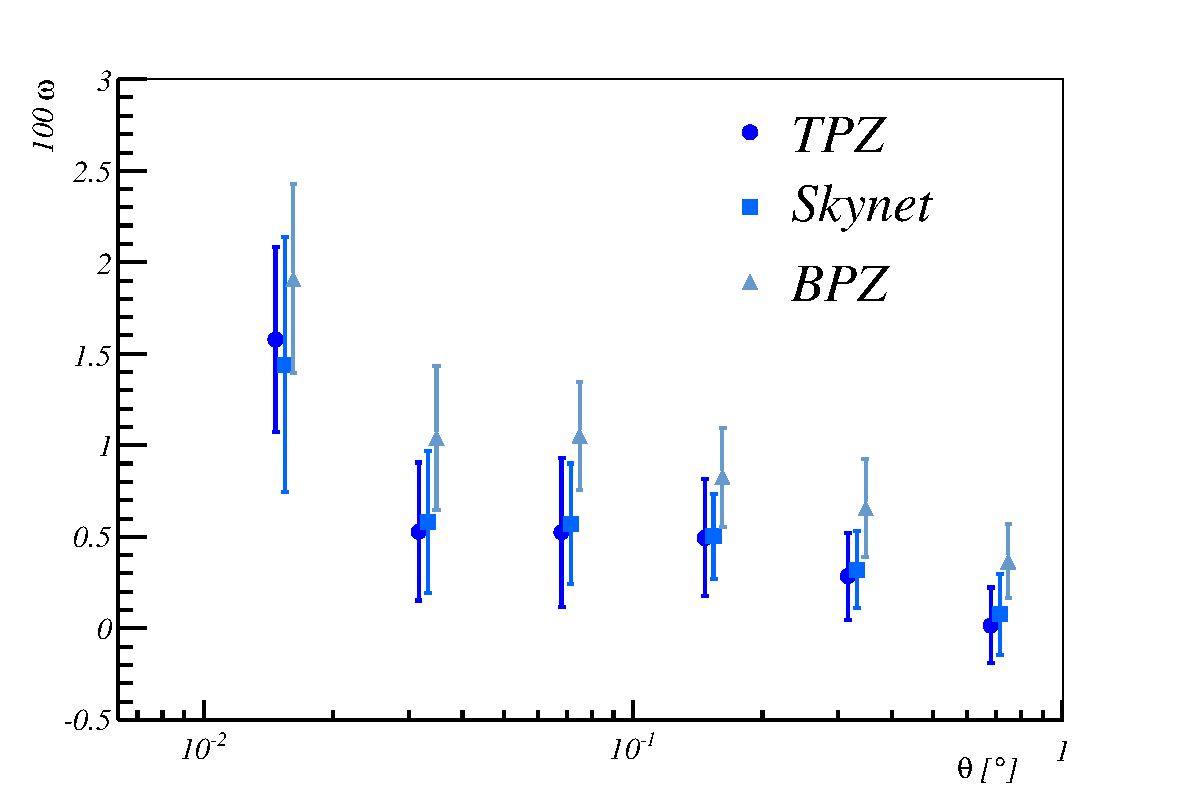
\includegraphics[width=0.75\textwidth]{./photoz_short.pdf}
\end{center}
\end{frame}
%%%%%%%%%%%%%%%%%%%%%%%%%%%%%%%%%%%%%%%%%%%%%%%%%%%%%%%%%%%%%%%%%%%%%%%%%
\begin{frame}[plain]
\begin{LARGE}
\begin{center}
{{\bf \color{blue}MAGNIFICATION DES-Y1}}
\end{center}
\end{LARGE}
\end{frame}
%%%%%%%%%%%%%%%%%%%%%%%%%%%%%%%%%%%%%%%%%%%%%%%%%%%%%%%%%%%%%%%%%%%%%%%%%
\begin{frame}
\frametitle{\begin{small}\underline{{\bf Magnification DES-Y1.}}\end{small}}
{\bf \color{red}The possible science with magnification:}\\
\vspace{0.2cm}
\begin{itemize}
\item Combination with other probes.\\
$\rightarrow$ Caution with systematic.\\
$\rightarrow$ Covariances reduce the impact on the measurement.
\vspace{0.2cm}
\item Search for new alternative and independent probes.\\
$\rightarrow$ {\bf The clever solution:}\\
Search for environments dominated by DE.
\begin{center}
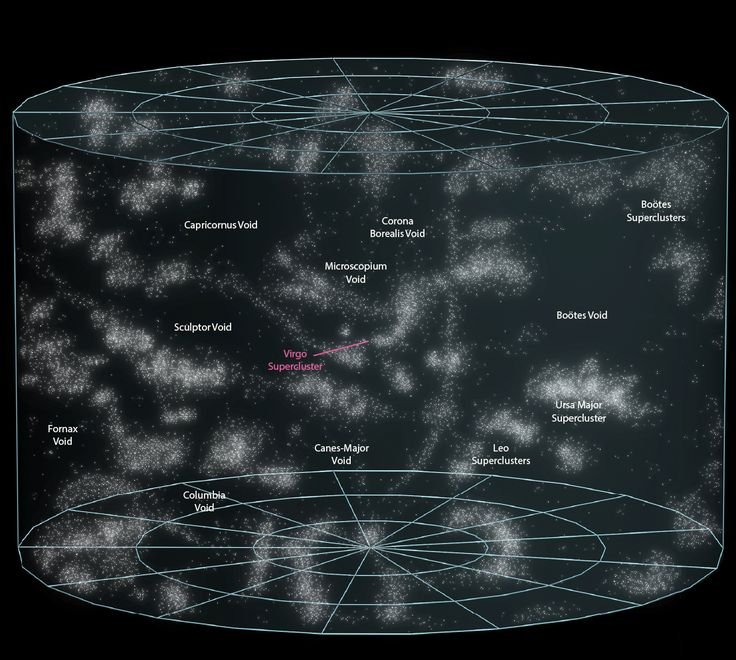
\includegraphics[width=0.4\textwidth]{./voids_local_universe.jpg}
\end{center}
\end{itemize}
\end{frame}
%%%%%%%%%%%%%%%%%%%%%%%%%%%%%%%%%%%%%%%%%%%%%%%%%%%%%%%%%%%%%%%%%%%%%%%%%
\begin{frame}
\frametitle{\begin{small}\underline{{\bf Magnification DES-Y1.}}\end{small}}
\begin{columns}
\column{0.02\textwidth}
\column{0.52\textwidth}
Dense sources allows low dense lenses:
\vspace{0.2cm}
\begin{itemize}
\item {\color{red}\bf Voids}.
\vspace{0.2cm}
\item Troughs.
\vspace{0.2cm}
\item Clusters.
\end{itemize}
\vspace{1cm}
{\bf Direct probe} of the matter profile.
\begin{center}
\end{center}
\column{0.55\textwidth}
\begin{center}
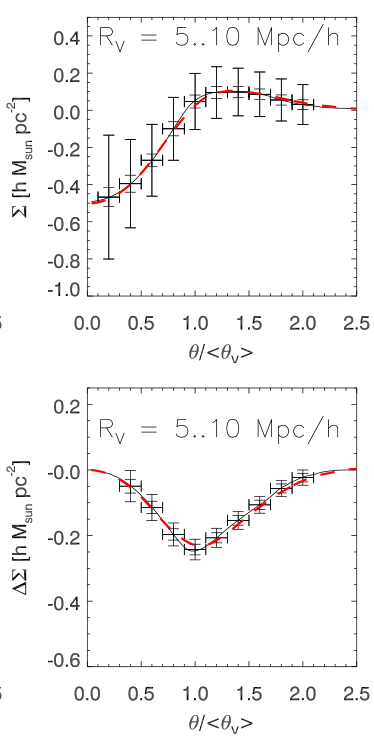
\includegraphics[height=0.8\textheight]{./figures/krause_void.png}\\
\begin{footnotesize}(arXiv:1210.2446)\end{footnotesize}
\end{center}
\end{columns}
\end{frame}
%%%%%%%%%%%%%%%%%%%%%%%%%%%%%%%%%%%%%%%%%%%%%%%%%%%%%%%%%%%%%%%%%%%%%%%%%
\begin{frame}
\frametitle{\begin{small}\underline{{\bf Magnification DES-Y1.}}\end{small}}
\begin{columns}
\column{0.45\textwidth}
\begin{center}
{\bf Trough gg-lensing.}\\
\vspace{0.3cm}
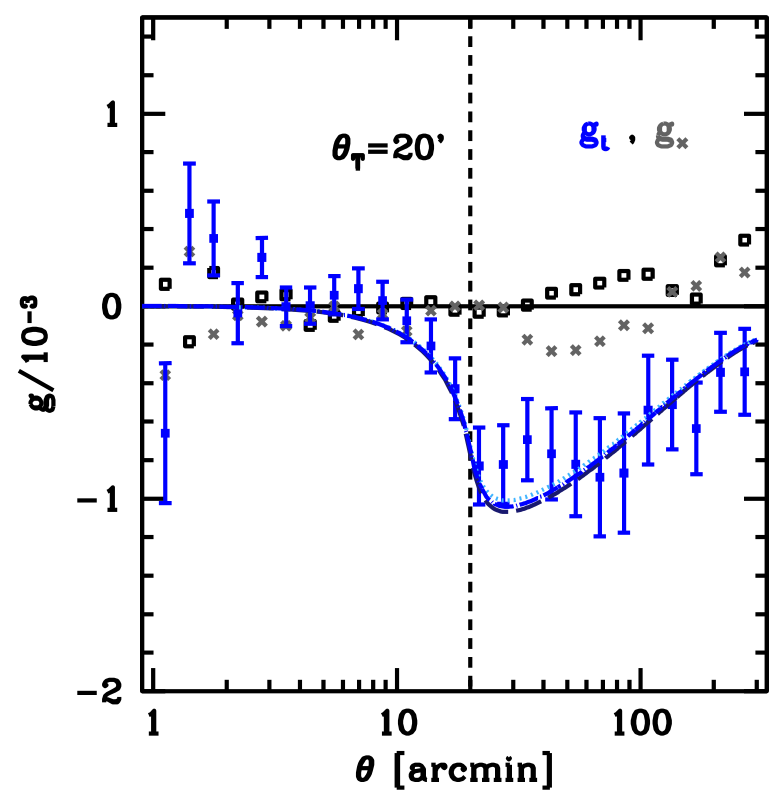
\includegraphics[width=0.8\textwidth]{./figures/gg-trough.png}\\
\begin{footnotesize}(arXiv:1507.05090)\end{footnotesize}
\end{center}
\column{0.5\textwidth}
\begin{center}
{\bf Void gg-lensing.}\\
\vspace{0.3cm}
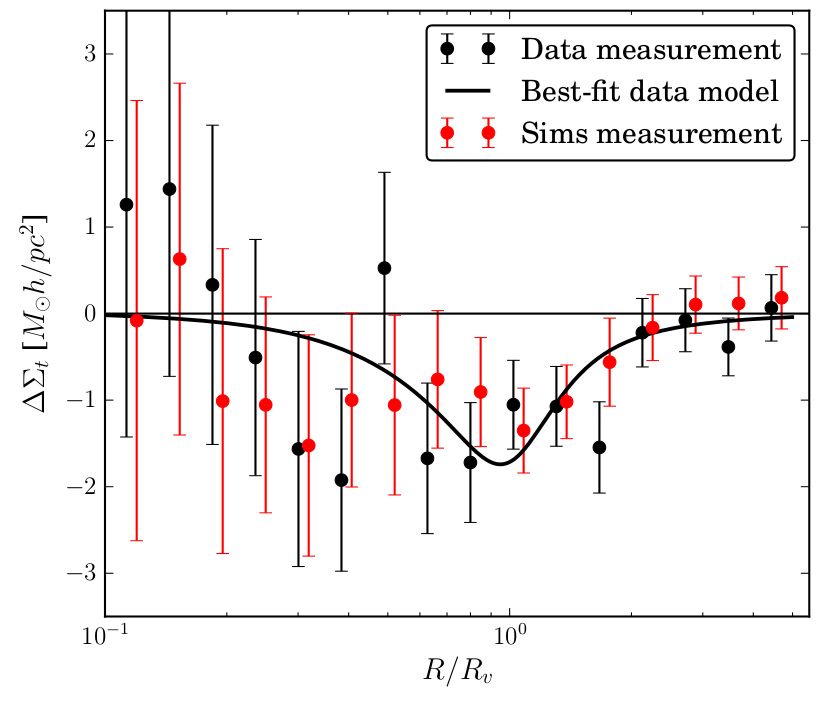
\includegraphics[width=0.8\textwidth]{./figures/gg-voids.png}\\
\begin{footnotesize}(arXiv:1605.03982)\end{footnotesize}
\end{center}
\end{columns}
\end{frame}
%%%%%%%%%%%%%%%%%%%%%%%%%%%%%%%%%%%%%%%%%%%%%%%%%%%%%%%%%%%%%%%%%%%%%%%%%
\begin{frame}
\frametitle{\begin{small}\underline{{\bf Magnification DES-Y1.}}\end{small}}
{\bf Void profile with Modified Gravity f(R) models.}
\begin{columns}
\column{0.5\textwidth}
\begin{center}
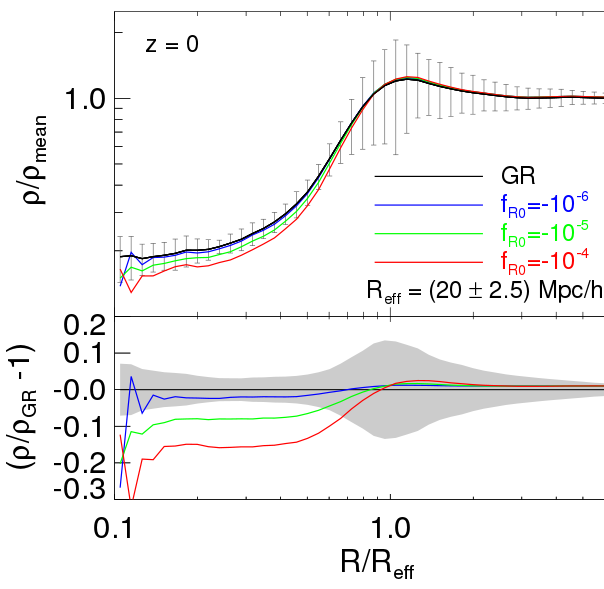
\includegraphics[width=0.8\textwidth]{./figures/void_fr.png}\\
\begin{footnotesize}(arXiv:1511.01494)\end{footnotesize}
\end{center}
\column{0.5\textwidth}
\begin{center}
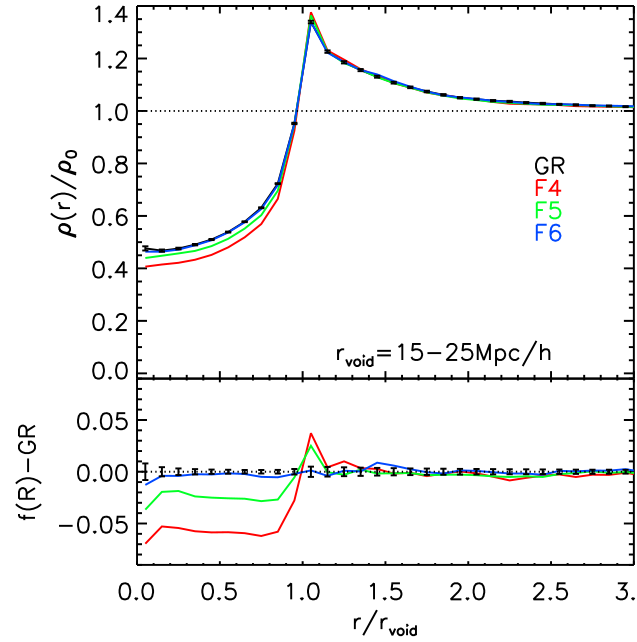
\includegraphics[width=0.8\textwidth]{./figures/void_fr2.png}\\
\begin{footnotesize}(arXiv:1410.8355)\end{footnotesize}
\end{center}
\end{columns}
\end{frame}
%%%%%%%%%%%%%%%%%%%%%%%%%%%%%%%%%%%%%%%%%%%%%%%%%%%%%%%%%%%%%%%%%%%%%%%%%
\begin{frame}
\frametitle{\begin{small}\underline{{\bf Magnification DES-Y1.}}\end{small}}
\begin{columns}
\column{0.5\textwidth}
{\bf The source data sample:} DES-Y1-Gold.\\
\vspace{0.2cm}
\begin{itemize}
\item S/G-separation: {\tt modest\_class} \& spread\_model\_i + 3$\times$spreaderr\_model\_i $>$ 0.007.
\vspace{0.2cm}
\item Depth: $i_{lim}> 22.0$ \& $i<20.5$.
\vspace{0.2cm}
\item Mask: worst 4\% \& bright-star halos removed.
\vspace{0.2cm}
\item $0.8 < z_{BPZ} < 1.5$.
\end{itemize}
\column{0.5\textwidth}
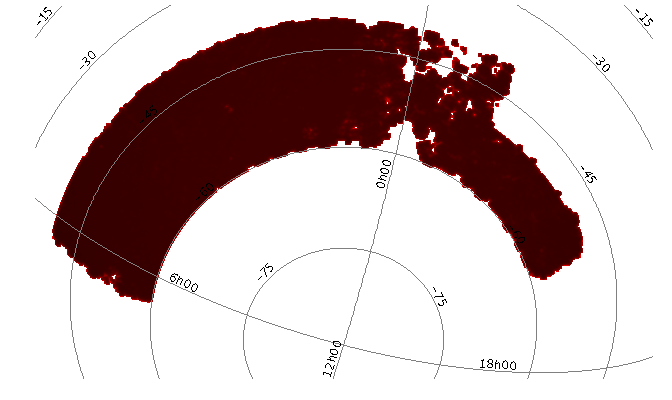
\includegraphics[width=\textwidth]{./masky1.png}
\end{columns}
\end{frame}
%%%%%%%%%%%%%%%%%%%%%%%%%%%%%%%%%%%%%%%%%%%%%%%%%%%%%%%%%%%%%%%%%%%%%%%%%
\begin{frame}
\frametitle{\begin{small}\underline{{\bf Magnification DES-Y1.}}\end{small}}
\begin{columns}
\column{0.5\textwidth}
{\bf Two lenses:} 
DES-Y1-redmagic.\\
$0.2 < z_{red} < 0.45$\\
\vspace{0.2cm}
\begin{itemize}
\item Voids.\\
\includegraphics[width=0.6\textwidth]{./voids_footprint.png}
\vspace{0.2cm}
\item Troughs.\\
\includegraphics[width=0.6\textwidth]{./trough_10_q0.png}
\end{itemize}
\column{0.5\textwidth}
\begin{center}
\includegraphics[width=0.75\textwidth]{./phiz_mag_auto_i1.png}\\
\includegraphics[width=0.7\textwidth]{./lognormal.png}
\end{center}
\end{columns}
\end{frame}
%%%%%%%%%%%%%%%%%%%%%%%%%%%%%%%%%%%%%%%%%%%%%%%%%%%%%%%%%%%%%%%%%%%%%%%%%
\begin{frame}
\frametitle{\begin{small}\underline{{\bf Magnification DES-Y1.}}\end{small}}
\includegraphics[width=\textwidth]{./troughs_ap10_mag_auto_i1.png}
\end{frame}
%%%%%%%%%%%%%%%%%%%%%%%%%%%%%%%%%%%%%%%%%%%%%%%%%%%%%%%%%%%%%%%%%%%%%%%%%
\begin{frame}
\frametitle{\begin{small}\underline{{\bf Magnification DES-Y1.}}\end{small}}
\includegraphics[width=\textwidth]{./troughs_ap20_mag_auto_i1.png}
\end{frame}
%%%%%%%%%%%%%%%%%%%%%%%%%%%%%%%%%%%%%%%%%%%%%%%%%%%%%%%%%%%%%%%%%%%%%%%%%
\begin{frame}
\frametitle{\begin{small}\underline{{\bf Magnification DES-Y1.}}\end{small}}
\includegraphics[width=\textwidth]{./troughs_ap30_mag_auto_i1.png}
\end{frame}
%%%%%%%%%%%%%%%%%%%%%%%%%%%%%%%%%%%%%%%%%%%%%%%%%%%%%%%%%%%%%%%%%%%%%%%%%
\begin{frame}
\frametitle{\begin{small}\underline{{\bf Magnification DES-Y1.}}\end{small}}
{\bf Theory:}\\
\vspace{0.2cm}
$\rightarrow$ Used Fiedrich et al. (in prep) and Gruen et al. (2016) theory.\\
\vspace{0.2cm}
$\rightarrow$ Planck 2015 parameters blinded.\\
\vspace{0.5cm}
{\bf Covariances:}\\
\vspace{0.2cm}
$\rightarrow$ Bootstrap resampling {\bf only} the lenses.
\end{frame}
%%%%%%%%%%%%%%%%%%%%%%%%%%%%%%%%%%%%%%%%%%%%%%%%%%%%%%%%%%%%%%%%%%%%%%%%%
\begin{frame}
\frametitle{\begin{small}\underline{{\bf Magnification DES-Y1.}}\end{small}}
{\bf Significance of detection:}\\
$\rightarrow$ Defined by the $\chi^2$ against zero.
\begin{center}
\begin{tabular}{c | c c c c c }
$\theta_T$& & &$10'$& &\\
$Q$&0&1&2&3&4\\
$\chi^2_z/ndof$ &43.5/7&10.5/7&1.3/7&10.3/7&45.3/7\\
\hline
\hline
$\theta_T$& & &$20'$& & \\
$Q$&0&1&2&3&4 \\
$\chi^2_z/ndof$&19.0/7&7.5/7&4.0/7&18.3/7&17.0/7\\
\hline
\hline
$\theta_T$& & &$30'$& & \\
$Q$&0&1&2&3&4\\
$\chi^2_z/ndof$&28.3/7&3.8/7&16.4/7&5.1/7&17.3/7\\
\end{tabular}
\end{center}
\end{frame}
%%%%%%%%%%%%%%%%%%%%%%%%%%%%%%%%%%%%%%%%%%%%%%%%%%%%%%%%%%%%%%%%%%%%%%%%%
\begin{frame}
\frametitle{\begin{small}\underline{{\bf Magnification DES-Y1.}}\end{small}}
\begin{center}
\includegraphics[width=0.7\textwidth]{./void_stacked_mag_auto_i1.png}
\end{center}
\end{frame}
%%%%%%%%%%%%%%%%%%%%%%%%%%%%%%%%%%%%%%%%%%%%%%%%%%%%%%%%%%%%%%%%%%%%%%%%%
\begin{frame}
\frametitle{\begin{small}\underline{{\bf Magnification DES-Y1.}}\end{small}}
{\bf Theory:}\\
\vspace{0.2cm}
$\rightarrow$ Used KGB (Kovacs \& Garcia-Bellido) profile.\\
\vspace{0.2cm}
$\rightarrow$ Planck 2015 parameters blinded.\\
\vspace{0.5cm}
{\bf Covariances:}\\
\vspace{0.2cm}
$\rightarrow$ Bootstrap resampling {\bf only} the voids.\\
\vspace{0.5cm}
{\bf Significance:}\\
$\rightarrow$ Defined by the $\chi^2$ against zero.
$$\chi^2_{zero}/ndof = 33.6/15$$
{\bf \color{red} First detection ever of void (de-)magnification.}
\end{frame}
%%%%%%%%%%%%%%%%%%%%%%%%%%%%%%%%%%%%%%%%%%%%%%%%%%%%%%%%%%%%%%%%%%%%%%%%%
\begin{frame}[plain]
\begin{LARGE}
\begin{center}
{{\bf \color{blue}CONCLUSIONS}}
\end{center}
\end{LARGE}
\end{frame}
%%%%%%%%%%%%%%%%%%%%%%%%%%%%%%%%%%%%%%%%%%%%%%%%%%%%%%%%%%%%%%%%%%%%%%%%%
\begin{frame}
\frametitle{\begin{small}\underline{{\bf Conclusions.}}\end{small}}
\begin{itemize}
\item Magnification is a powerful probe for the matter profile.
\vspace{0.3cm}
\item Combined with gg-lensing provide good systematic control.
\vspace{0.3cm}
\item A new technique to measure magnification has been developed.
$\rightarrow$Including a novel way to deal with systematic errors.
\vspace{0.3cm}
\item Magnification allows access to lowest voids scales
\vspace{0.3cm}
\item Lowest void scales provide constrains on Modified Gravity scenarios.
\vspace{0.3cm}
\item {\color{red}First direct measurement} of a void convergence profile.\\
$\rightarrow$Opens a new window to probe the dark Universe!
\end{itemize}
\end{frame}
%%%%%%%%%%%%%%%%%%%%%%%%%%%%%%%%%%%%%%%%%%%%%%%%%%%%%%%%%%%%%%%%%%%%%%%%%
\end{document}
